
\documentclass[9pt,twocolumn,twoside]{pnas-new}
\usepackage{multirow} 
% Use the lineno option to display guide line numbers if required.

\templatetype{pnasinvited} % Choose template
% {pnasresearcharticle} = Template for a two-column research article
% {pnasmathematics} = Template for a one-column mathematics article
% {pnasinvited} = Template for a PNAS invited submission

\begin{document}

\title{Where Will Your Paper Go? Predicting Journal Submission and Citations with Topic Models}

% Use letters for affiliations, numbers to show equal authorship (if applicable) and to indicate the corresponding author
\author[a,1]{Zhe Guan}

\affil[a]{The University of Southampton}


% Please give the surname of the lead author for the running footer
\leadauthor{Zhe Guan}

% Please include corresponding author, author contribution and author declaration information
%\authorcontributions{Please provide details of author contributions here.}
%\authordeclaration{Please declare any competing interests here.}
\correspondingauthor{\textsuperscript{1}  E-mail: zg2u24\@soton.ac.uk}

% At least three keywords are required at submission. Please provide three to five keywords, separated by the pipe symbol.
\keywords{Topic Modeling $|$ Machine Learning $|$ Citation Prediction $|$ Journal Classification}

\begin{abstract}
%Citation and target journal prediction are of importance for academic scholars and government departments in guiding funding arrangements and research priority. Topic modelling of abstracts serves as an effective method to summarise the main idea of papers, providing a significant feature for citation and target journal prediction. In this study, we analysed papers from three different journals, applying various topic modelling techniques to improve the prediction performance of citations and target journals. 

Academic impact prediction is an important task for academic scholars, funding agencies, and journal editors to guide funding arrangements, research priorities, and editorial decisions. This study presents a framework that combines topic modelling techniques, including structural topic modelling (STM) and latent Dirichlet allocation (LDA), with machine learning classifiers while integrating multiple clustering algorithms, such as K-means and hierarchical clustering, to predict both the number of citations a paper will receive and the most suitable journal for submission. Additionally, an interactive dashboard tool is provided to allow users to input paper abstracts and obtain predictions using different models.

\end{abstract}

\dates{This manuscript was compiled on \today}
\doi{\url{https://github.com/phy-guanzh/Paper_Journal_Classification}}


\maketitle
\thispagestyle{firststyle}
\ifthenelse{\boolean{shortarticle}}{\ifthenelse{\boolean{singlecolumn}}{\abscontentformatted}{\abscontent}}{}

\section*{Introduction}

The exponential growth in the number of academic papers in different journals and on various topics brings unignorable challenges for researchers and policymakers who arrange funding and research priorities in institutions\cite{10.1162/qss_a_00327}. There is an increasing need for intelligent tools that can analyse and predict both citation potential and appropriate target journals for academic papers\cite{10.1002/asi.24810}. To address this, we focus on three journals within the field of operations research and systems analysis: the \href{ https://www.tandfonline.com/journals/tjor20}{``Journal of the Operational Research Society''}, \href{ https://www.tandfonline.com/journals/thss20}{``Health Systems''}, \href{https://www.tandfonline.com/journals/tjsm20}{``Journal of Simulation''}. The journals were selected for their relevance to decision analytics, healthcare systems, and simulation methodologies.

%In this work, three different journals, \href{ https://www.tandfonline.com/journals/tjor20}{``Journal of the Operational Research Society''}, \href{ https://www.tandfonline.com/journals/thss20}{``Health Systems''}, \href{https://www.tandfonline.com/journals/tjsm20}{``Journal of Simulation''} are compared and focused on. 


\section{Dataset and Cleaning}
The analysed dataset in this work includes the 4141 records. The initial features are shown in Table~\ref{tab:table1}.

\begin{table}[!htbp]
\centering
\caption{The initial features in dataset from journals}
\begin{tabular}{lr}
\toprule
Features & Description  \\
\midrule
Title & Title of the paper  \\
Journal & Name of the journal  \\
Year & Published year \\
Pages & Number of pages in the paper \\
Authors & Names of the authors \\
Views & Number of views the paper received \\
Citations & Number of times the paper was cited \\
Altmetric Score & Altmetric score indicating social and public engagement \\
Abstract & Summary of the paper's content \\
\bottomrule
\end{tabular}
\label{tab:table1}
\end{table}

Since the title name may reveal useful information for topic modelling, the two variables, ``Title'' and ``Abstract,'' are combined into a single input variable ``Title Abstract''. And ``Authors'' are transformed into ``Author\_Counts'' which can provide more useful information. Different techniques are applied to fill the missing 'Views' values in the train and test data, with details provided in the regression section. Considering that one of our targets is predicting journal names, the two variables, the ``Views'' and ``Almetric Score,'' are excluded from the model from the classification model, as these metrics are not available prior to submission.  A unique identifier, ``row\_id'', was added to each record.  ``Title\_Abstract'' was transformed into lemmatisation to standardise word forms first. Next, stop words and numeric tokens were removed to reduce noise in the dataset.

\section{Topic Modelling}
\subsection*{Bag of words and Comparisions} \

\noindent The combined text was tokenised into individual words and bigrams using a bag-of-words(BoW) approach~\cite{8950616}. The top 100 frequencies of unigrams and bigrams in the dataset are shown in Figure~\ref{fig:bagwords}. The bigrams can provide more information about differences among journals compared to common unigrams.

\begin{figure}[!tbhp]
\centering
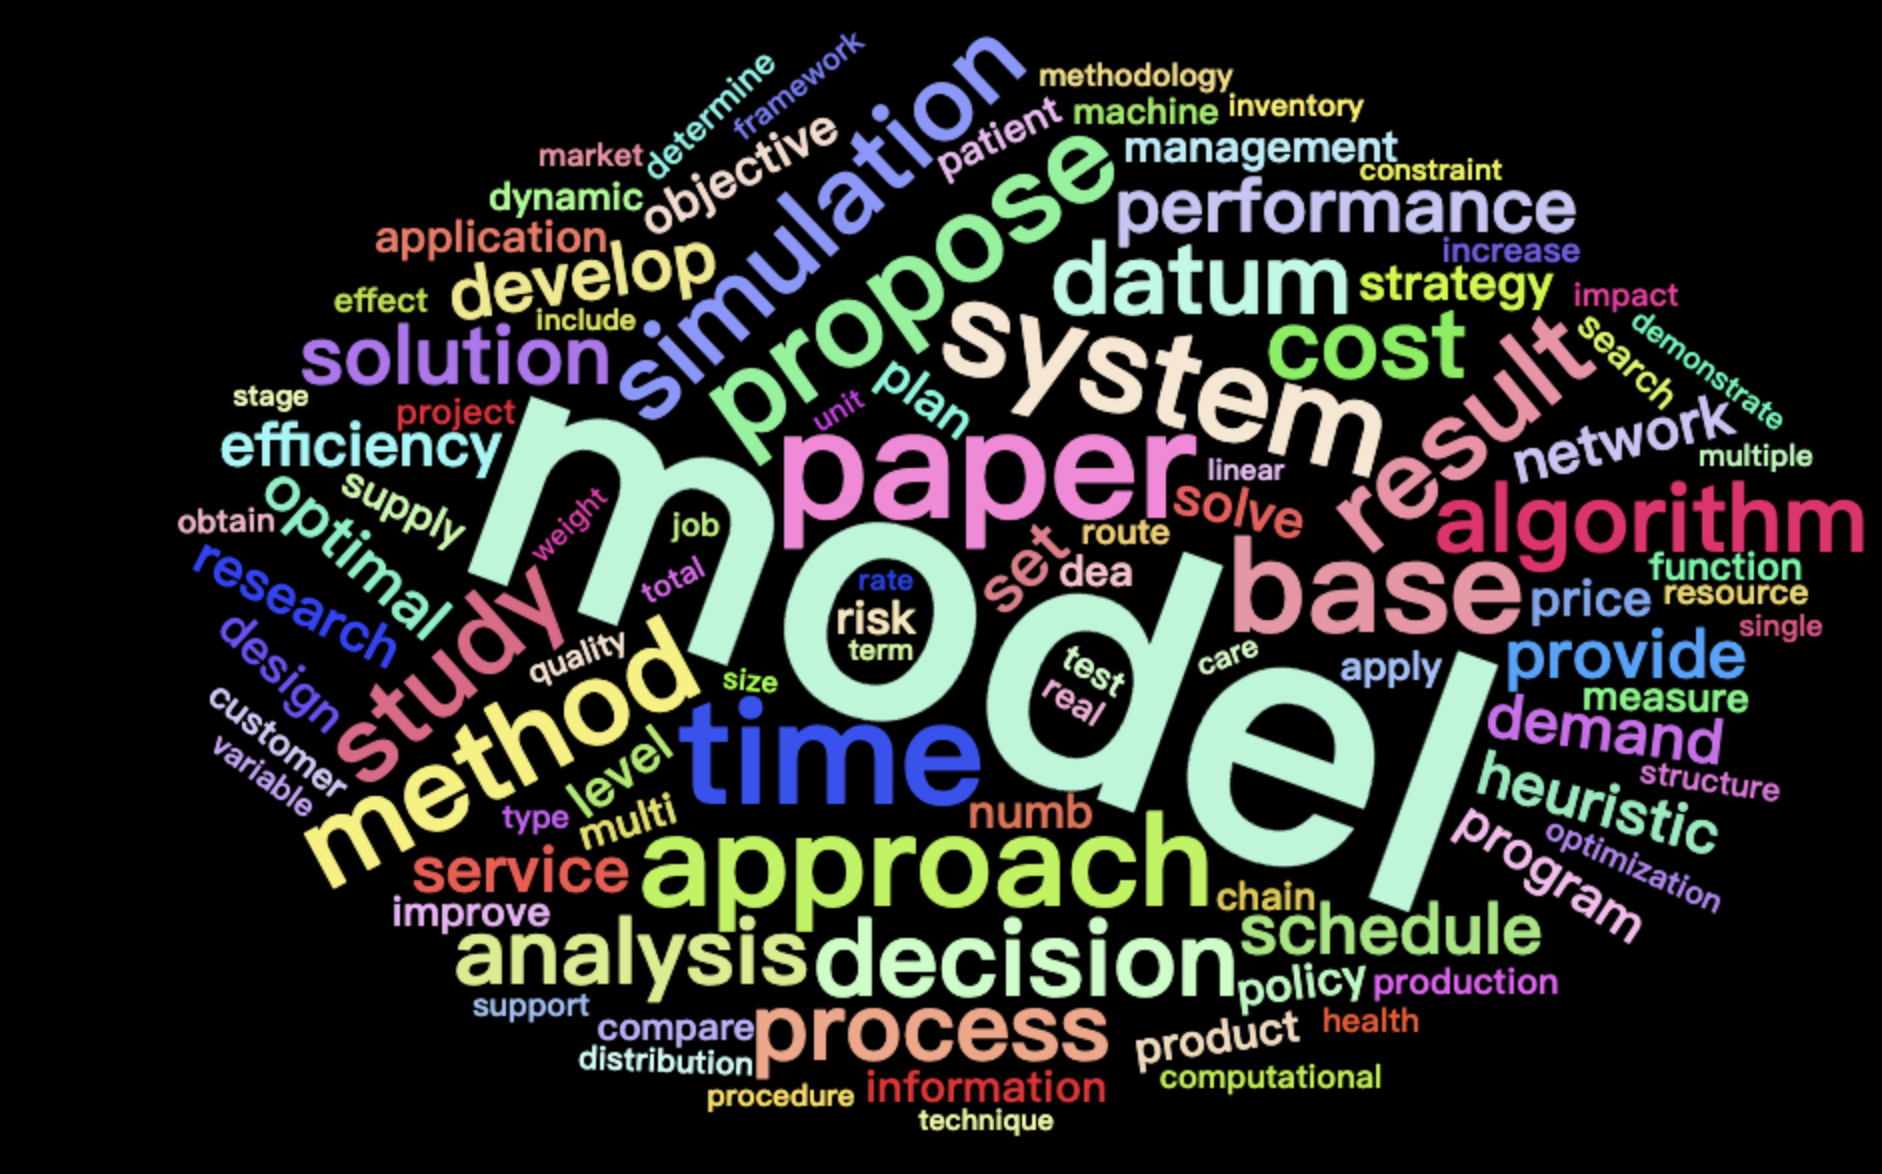
\includegraphics[width=0.4\linewidth]{bag_words/unigrams.png}
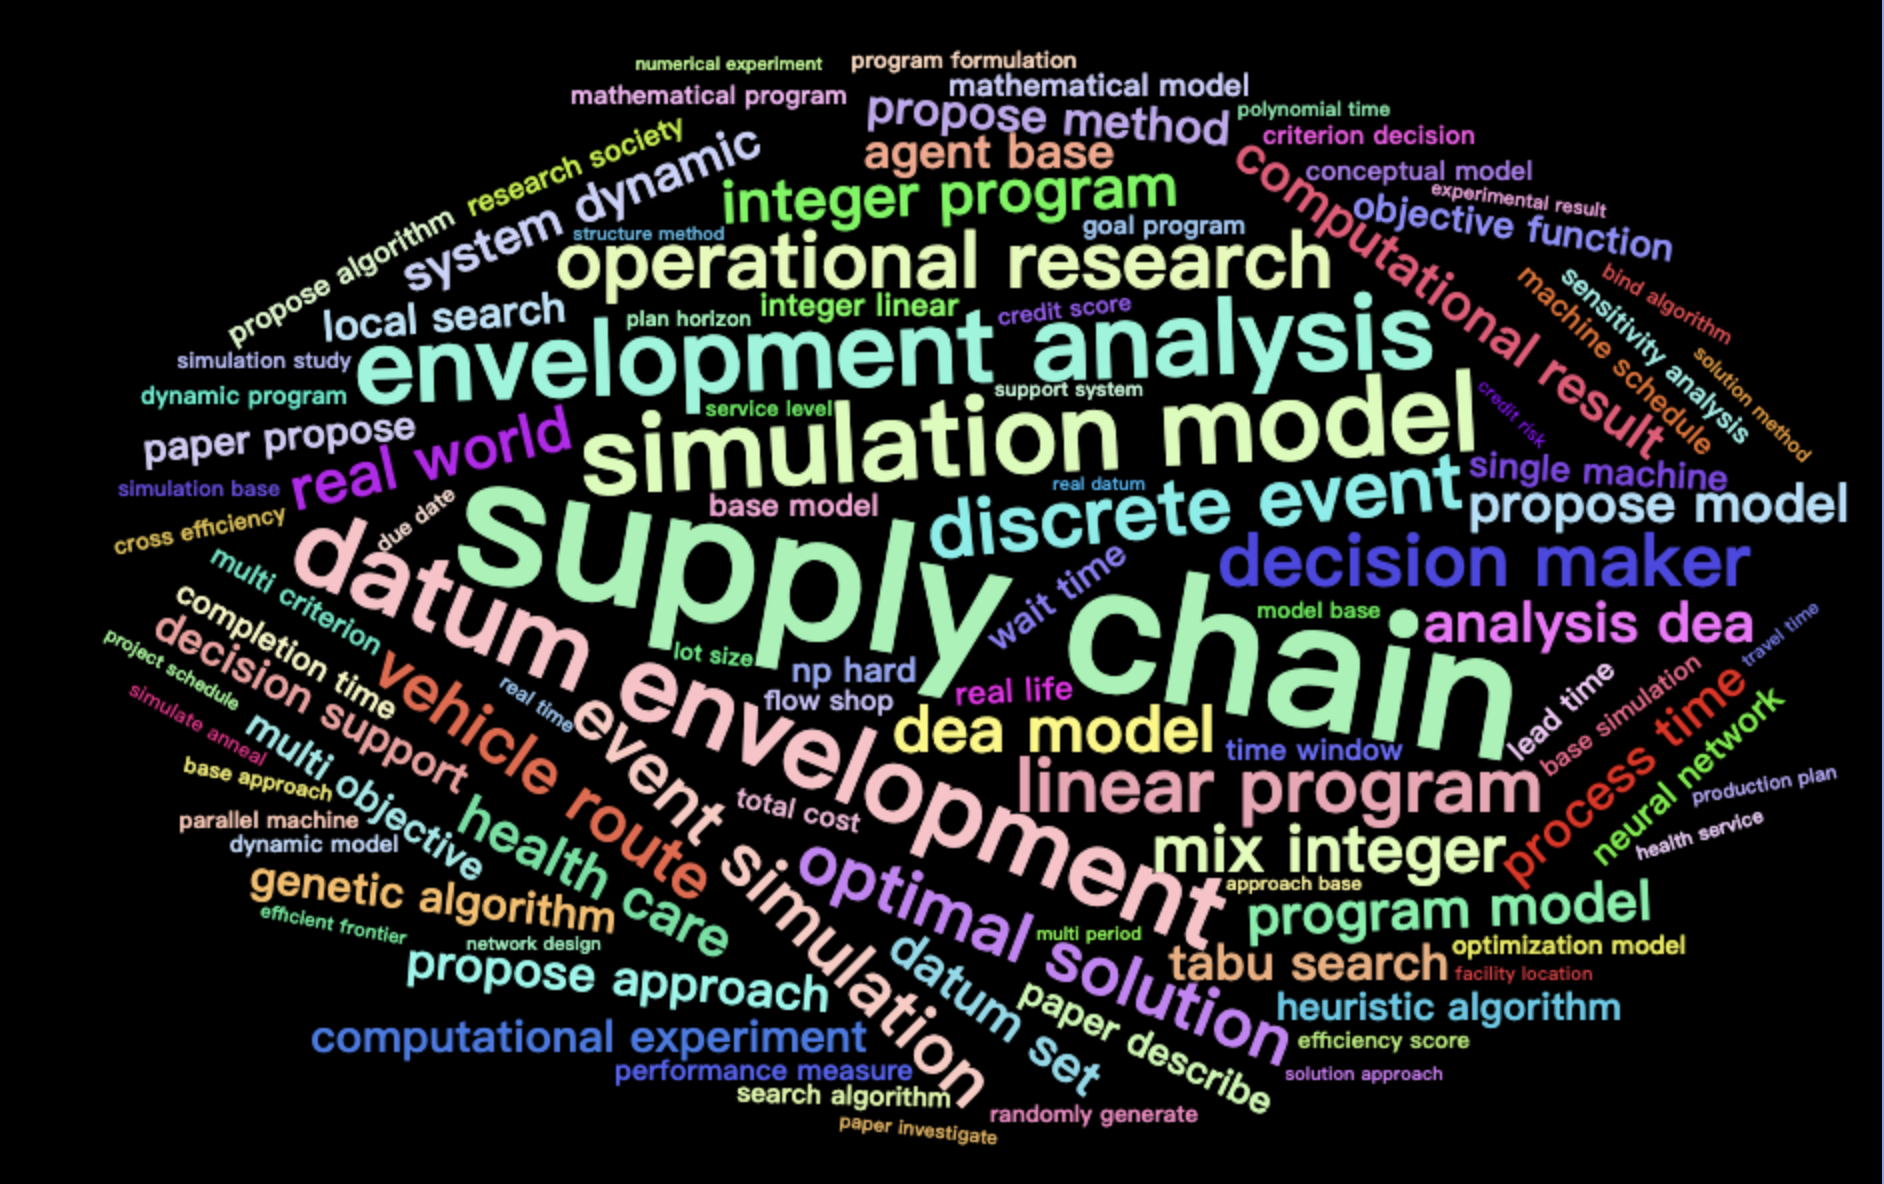
\includegraphics[width=0.4\linewidth]{bag_words/bigrams.png}
\caption{Top 100 frequencies of unigrams and bigrams from datasets}
\label{fig:bagwords}
\end{figure}
 
The BoW frequency of bigrams is analysed from two perspectives: its variation across different journals and over four time periods, as shown in Figure~\ref{fig:bagwordsjournal} and Figure~\ref{fig:bagwordstime}.

\begin{figure}[!tbhp]
\centering
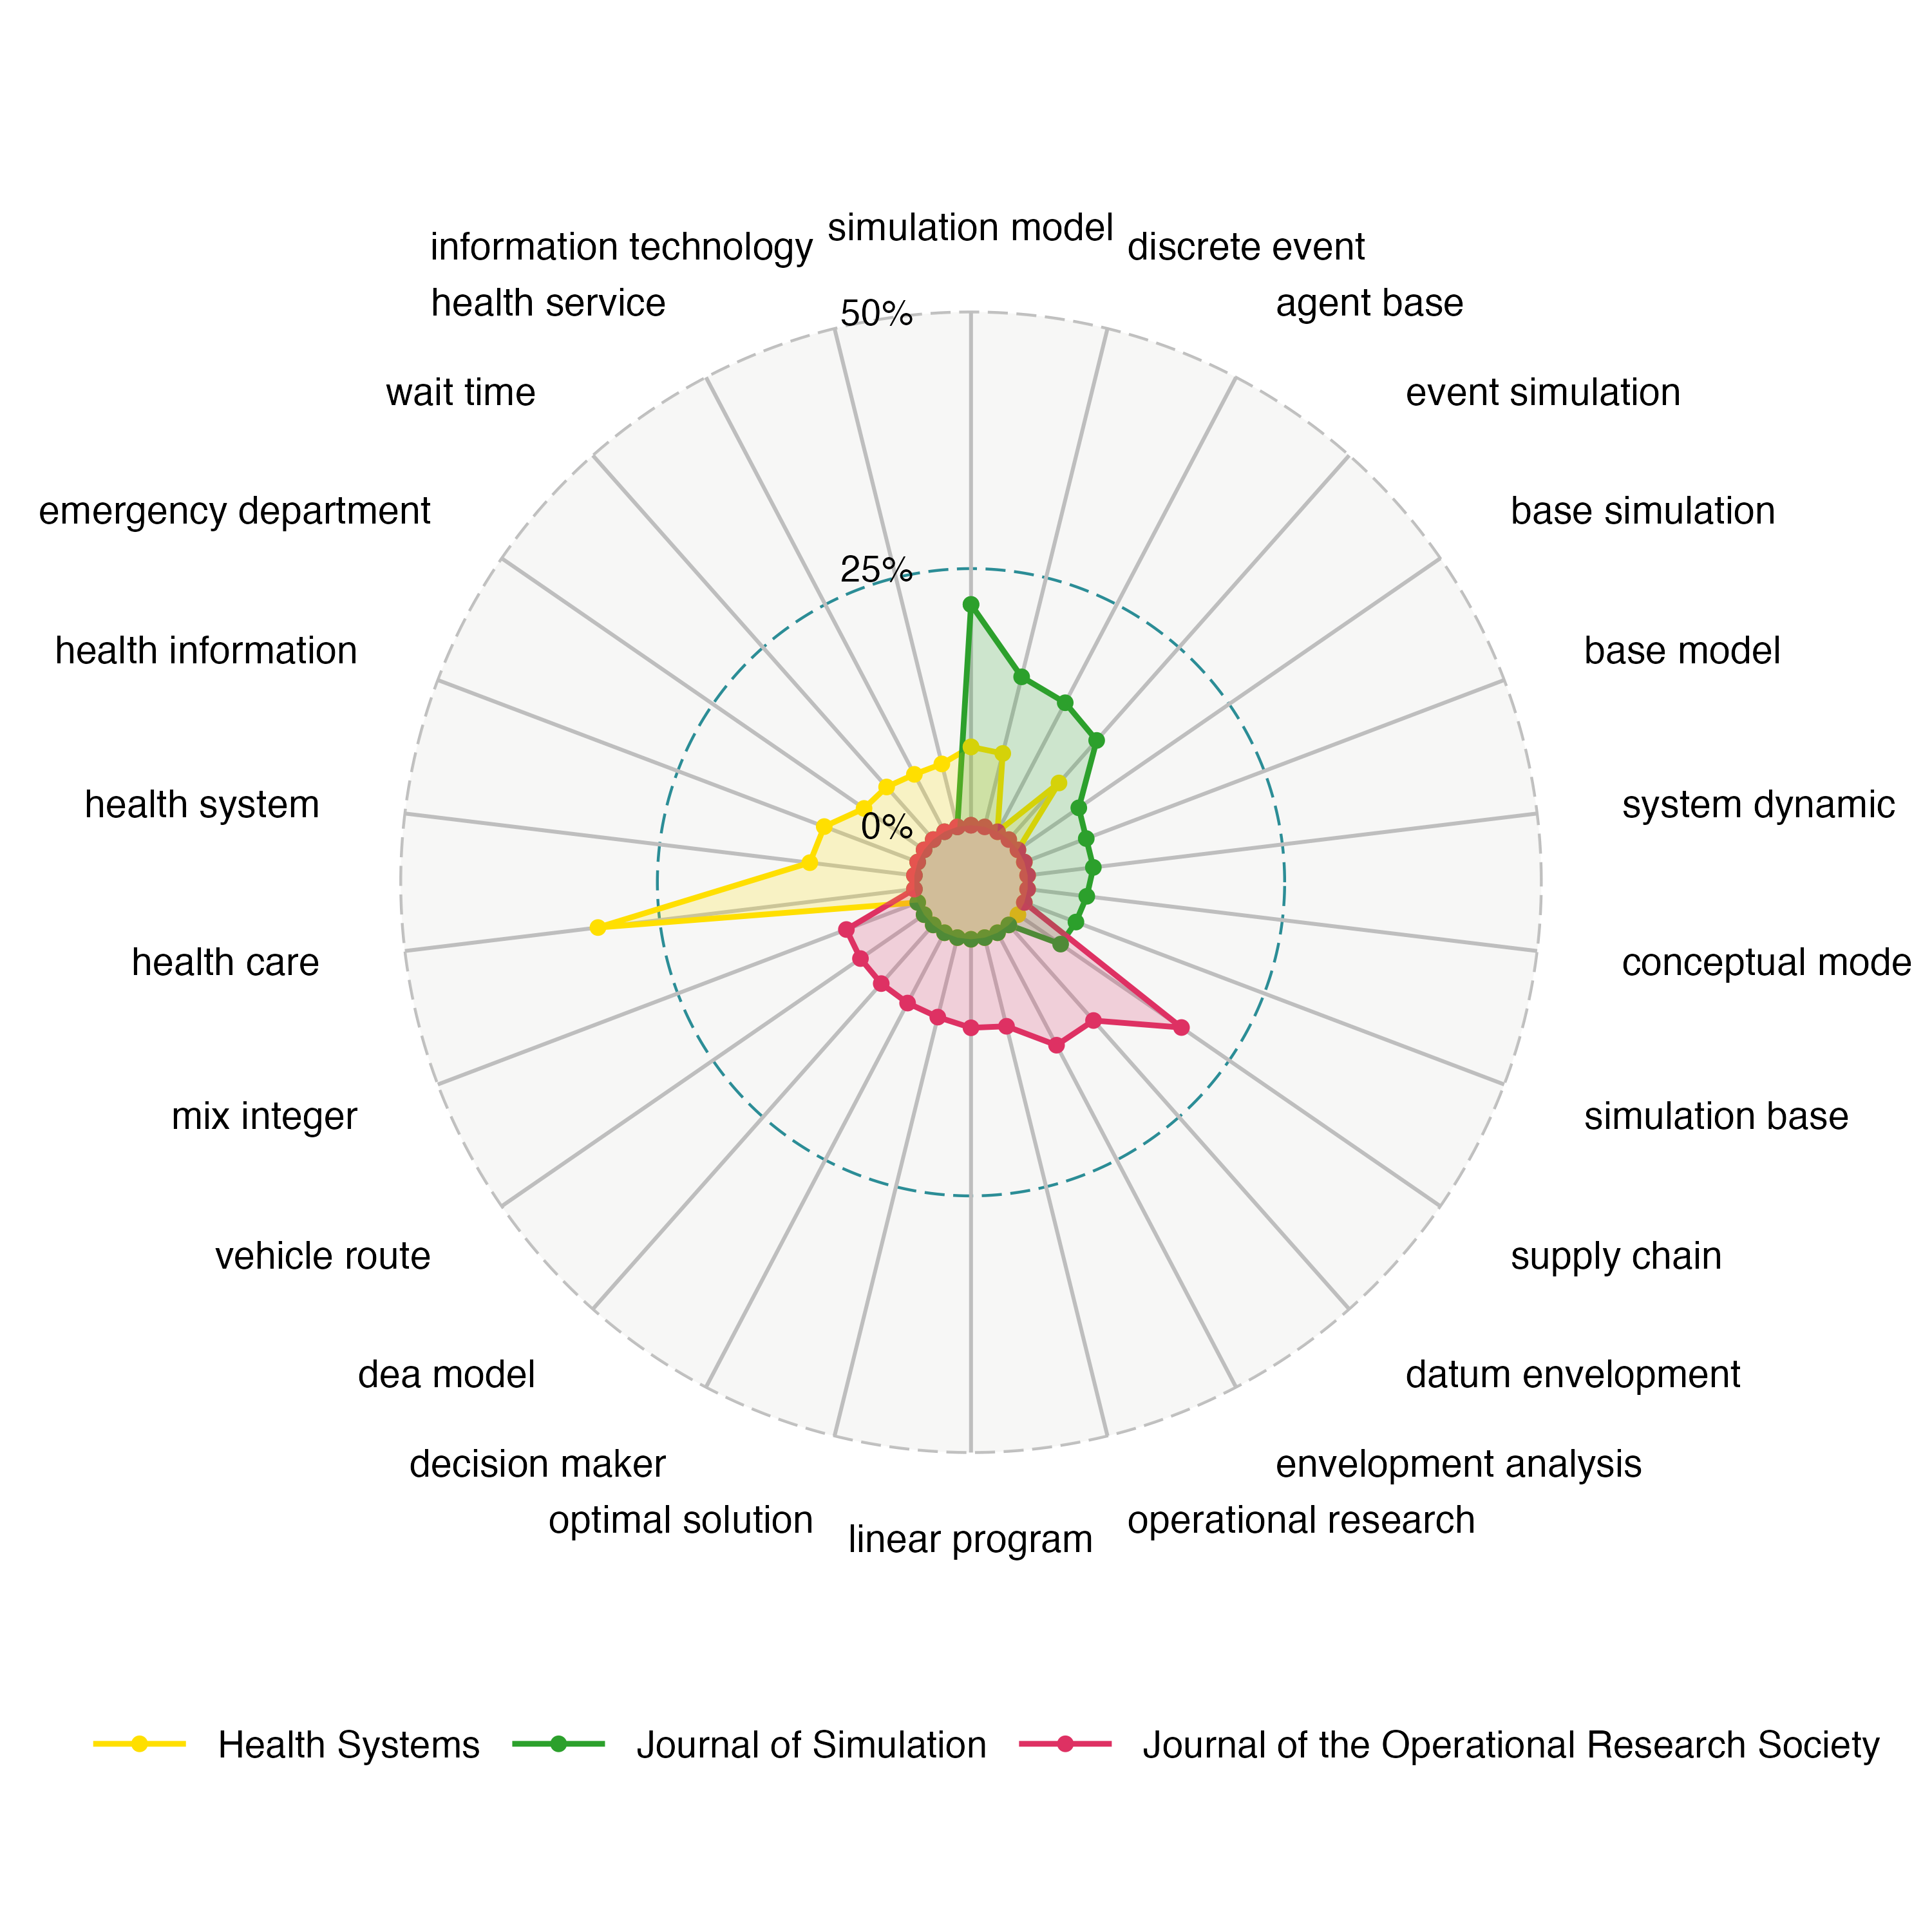
\includegraphics[width=0.3\textwidth]{bag_words/radar_journal.png}

\caption{The top 10 most frequent bigrams across three journals.}
\label{fig:bagwordsjournal}
\end{figure}

Different areas are focused on across journals, and the high-frequency bigrams show obvious distinctions, which can help in developing future classification models to identify the most appropriate target journal. Some common bigrams still exist across journals, such as ``simulation model'' and ``event simulation'' appearing between the journal \textit{Health Systems} and \textit{Journal of Simulation}, as well as ``supply chain'' shared between \textit{Journal of Simulation} and \textit{Journal of Operational Research Society}.

\begin{figure}[!tbhp]
\centering
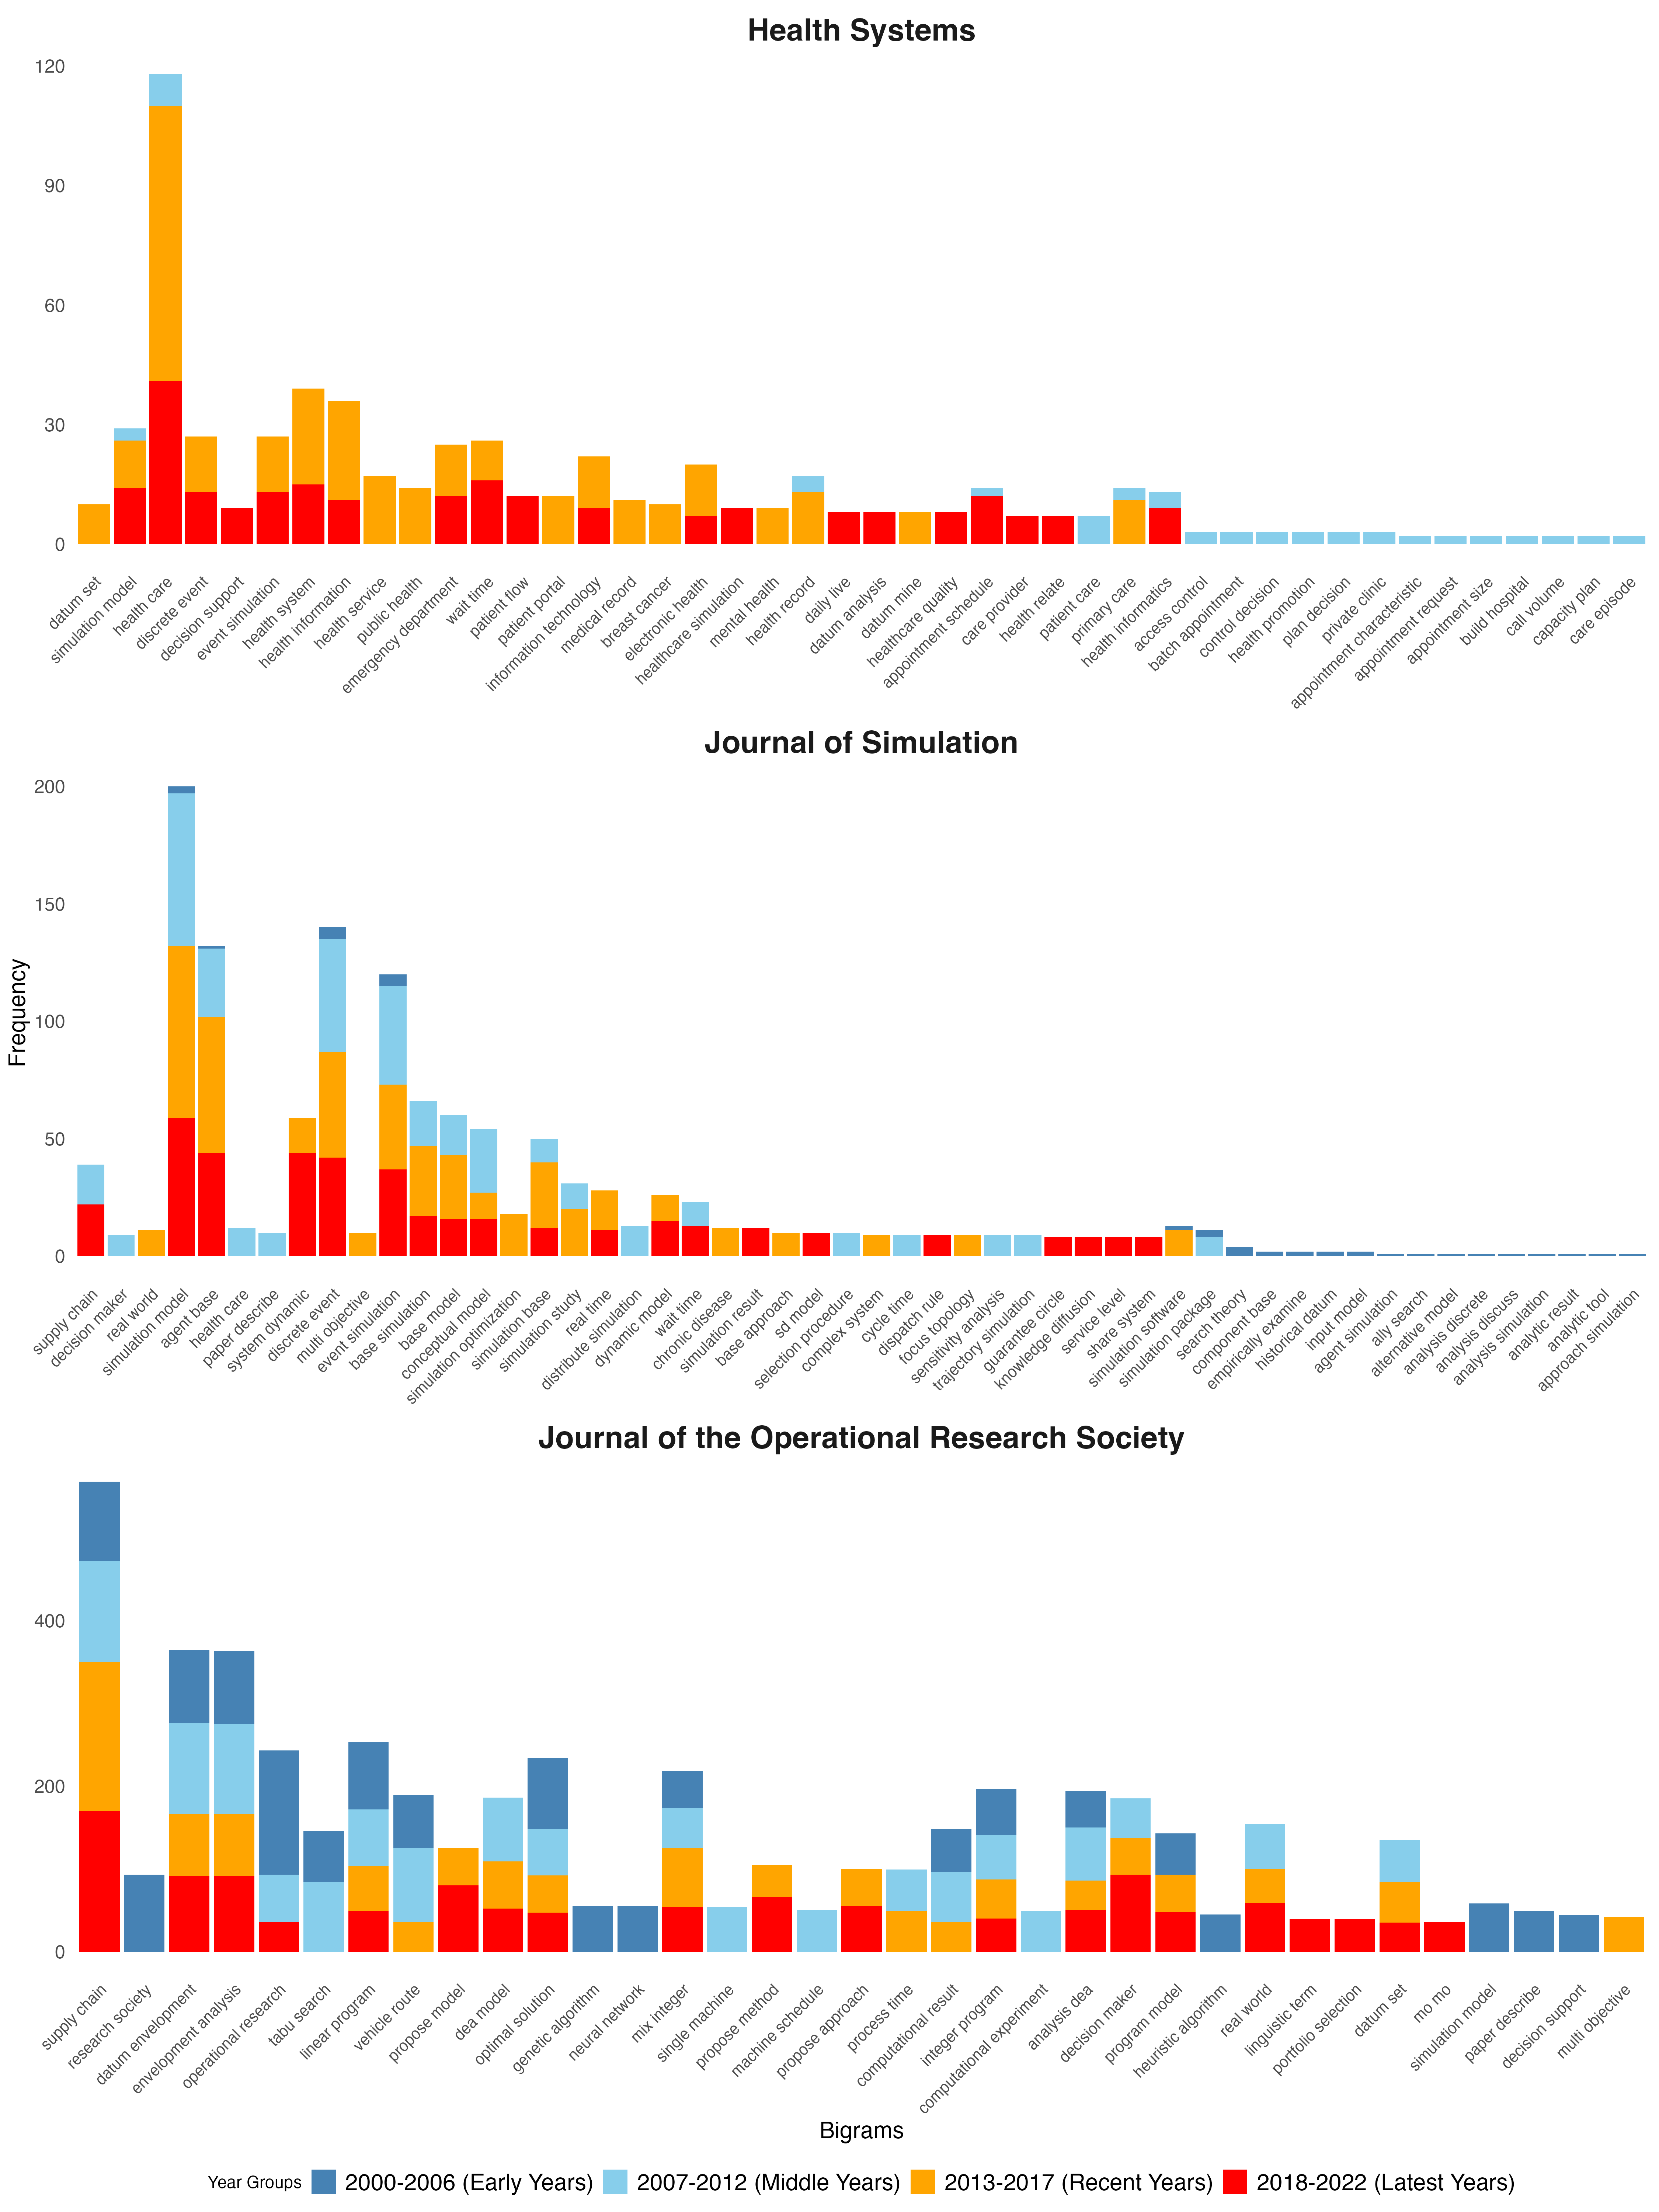
\includegraphics[width=0.42\textwidth]{bag_words/hist_journals_fre.png}

\caption{The top 30 most frequent bigrams from the dataset across four different time periods: 2000–2006, 2007–2012, 2013–2017, and 2018–2022 for three journals.}
\label{fig:bagwordstime}
\end{figure}

Some interesting phenomena appear over time across three journals. Firstly, there is no paper published in the journal \textit{Health Systems} before the Middle period (2007-2012), and ``health care'' is the main topic of the journal and shows increasing popularity across years. Secondly, the key bigrams in the \textit{Journal of Simulation} are relatively concentrated and increasingly popular across years, such as ``simulation model'', ``discrete event'', and ``event simulation'', whereas the \textit{Journal of the Operational Research Society} shows more flat probabilities across bigrams, with more focus on terms like "supply chain."


\subsection*{Latent Dirichlet Allocation} Latent Dirichlet Allocation (LDA)~\cite{10.4108/eai.13-7-2018.159623} is a widely used topic modelling algorithm that identifies hidden topics in a collection of documents based on word co-occurrence patterns. It assumes that each document is a mixture of topics, and each topic is a distribution over words. LDA requires specifying a value of \textit{k} (the number of topics) in the corpus as shown in Figure~\ref{fig:perplexityk6}. Determining an appropriate value for \textit{k} is significant, as it probably impacts the quality and interpretability of the topic modelling results. 


\begin{figure}[!tbhp]
\centering

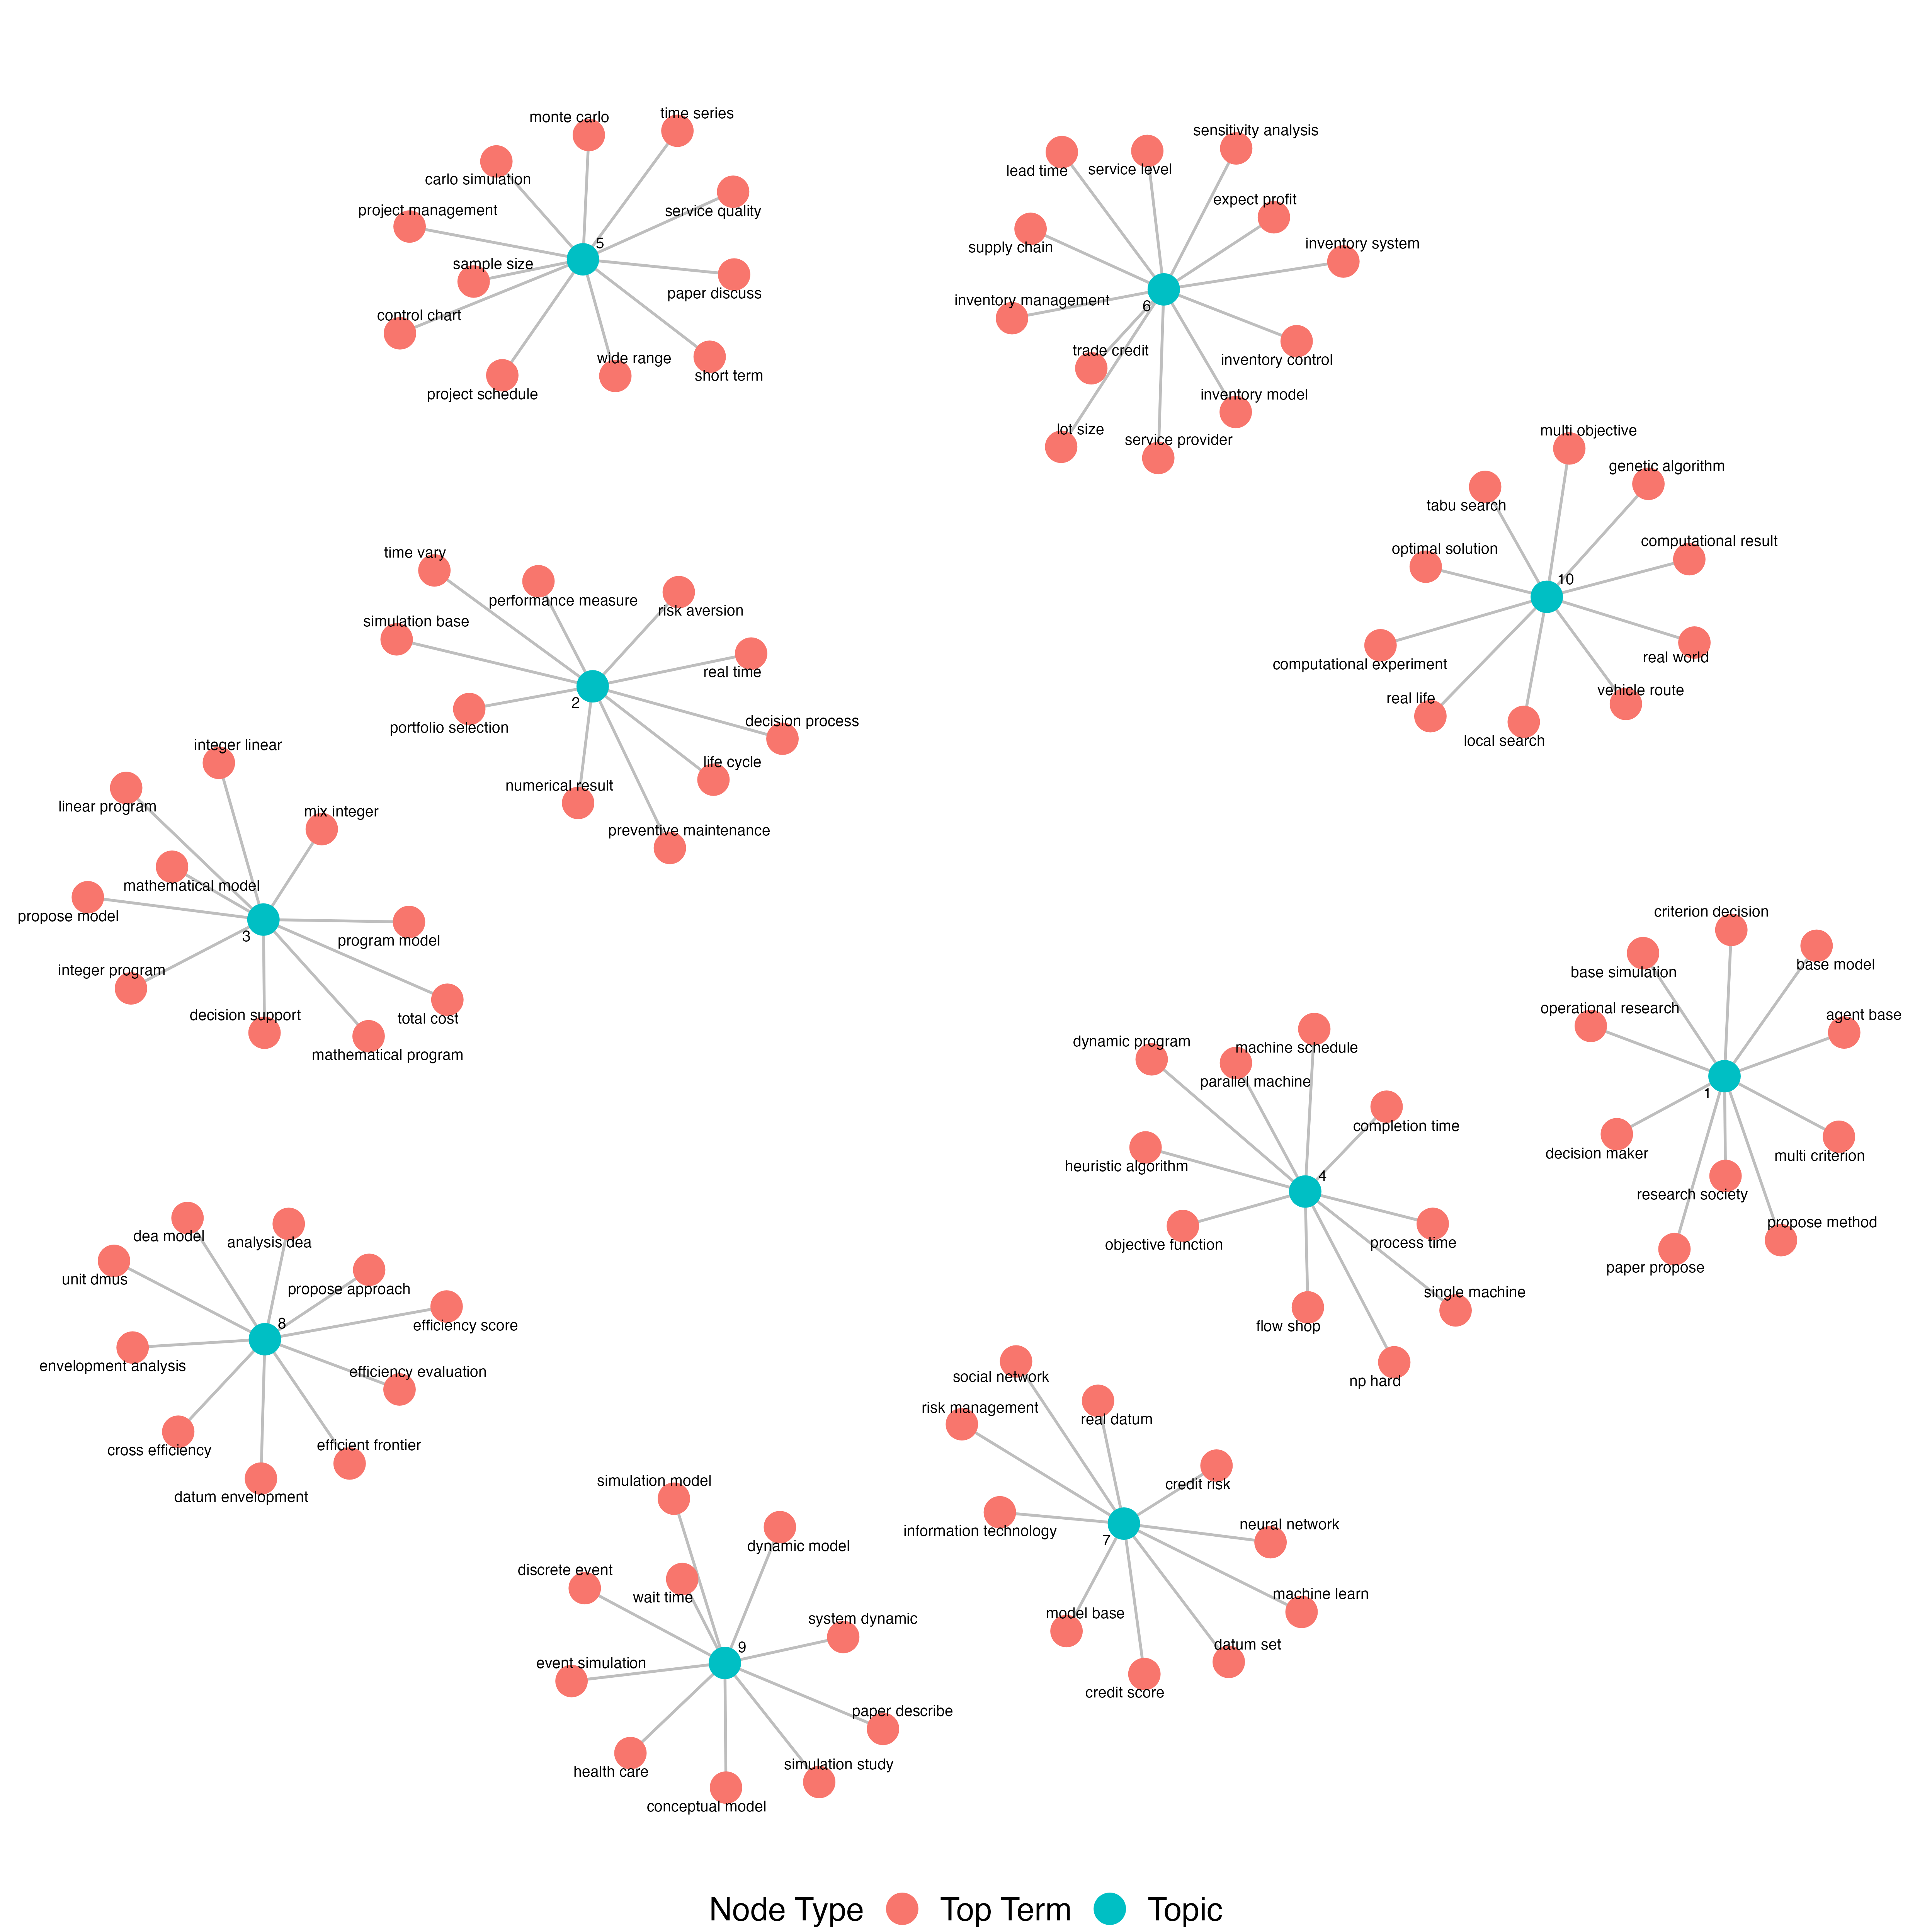
\includegraphics[width=0.9\linewidth]{bag_words/Topics_LDAk6.png}


\caption{The identified topics using LDA with the number of topics $k = 10$.}
\label{fig:perplexityk6}
\end{figure}



Perplexity is a common metric used to evaluate the fit of topic models and provides a reference for selecting the optimal \textit{k} value in LDA. 

Lower perplexity generally indicates a better model fit. As shown in Figure~\ref{fig:perplexity}, the \textit{2000-2022} year group has a much higher perplexity compared to other year groups, indicating that over a longer time span, the data is more diverse, and the model finds it harder to capture consistent topics across the entire period. Similarly, the \textit{Journal of the Operational Research Society} has a much higher perplexity compared to other journals, indicating that the journal covers a broader and more diverse range of topics, making it harder for the model to find consistent patterns.

Furthermore, Figure~\ref{fig:perplexity} also shows that considering dataset features can help reduce perplexity and the optimal number of topics.


\begin{figure}[!tbhp]
\centering

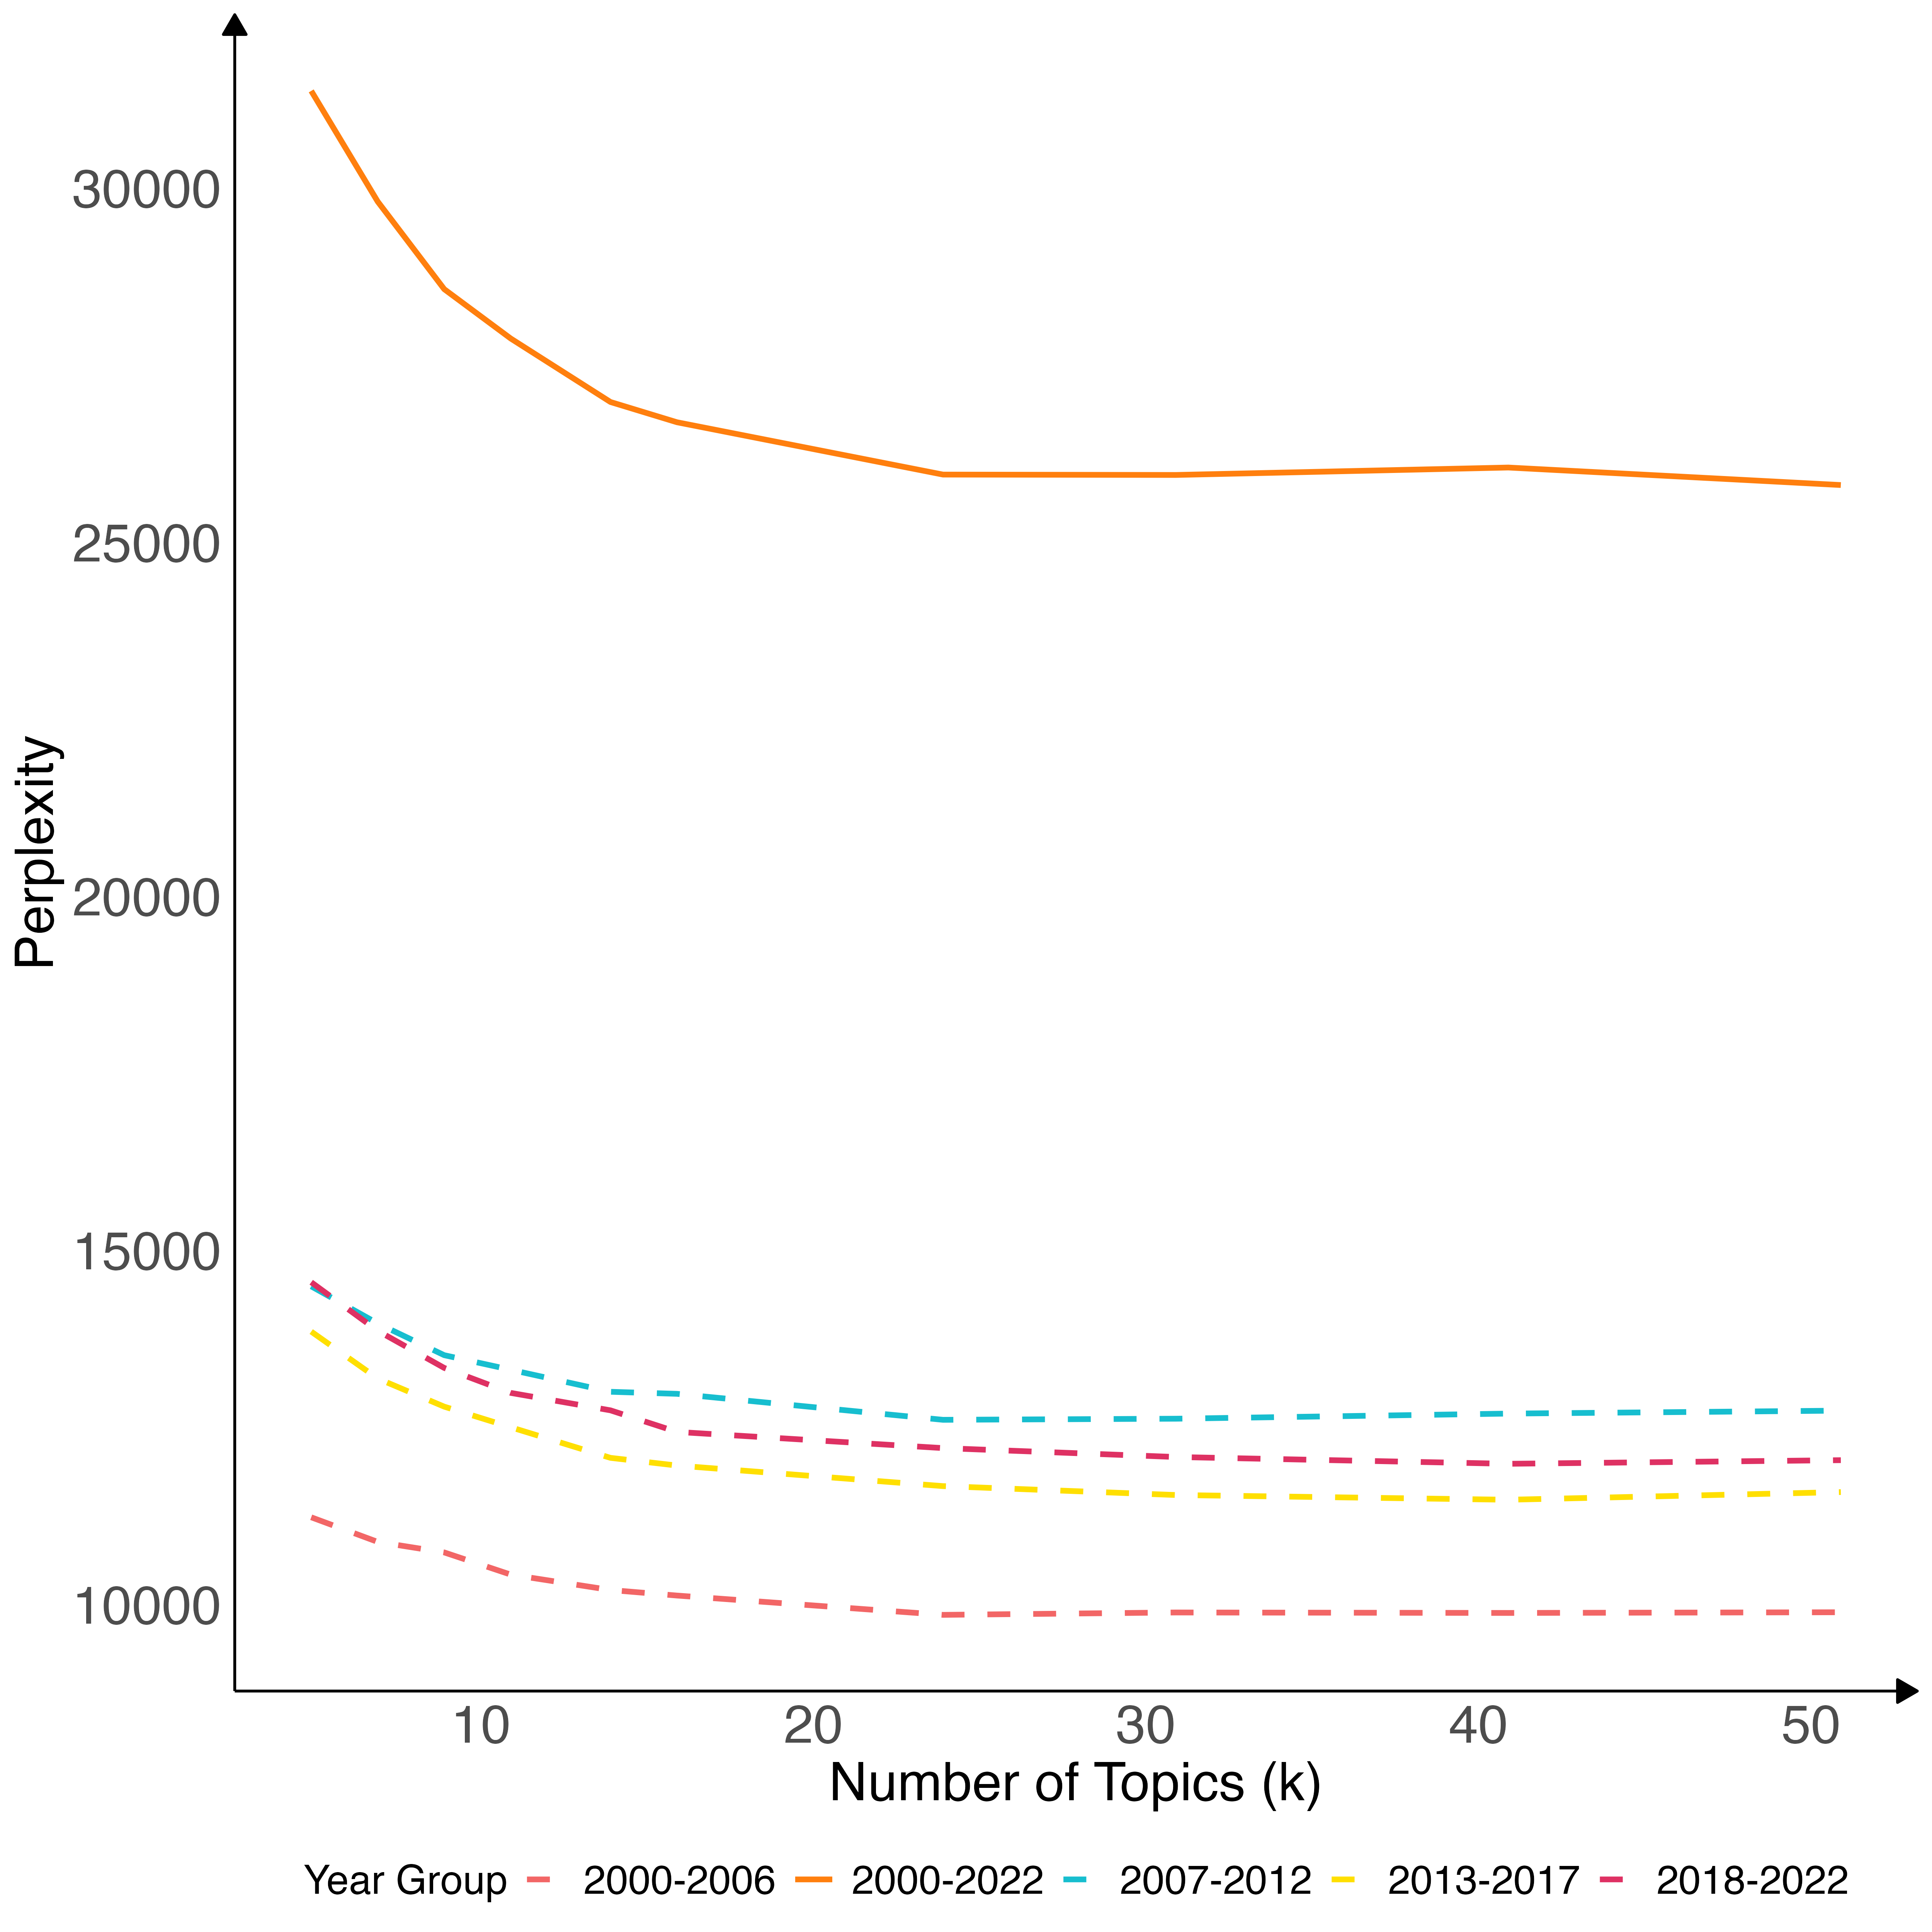
\includegraphics[width=0.49\linewidth]{bag_words/Perplexity_year.png}
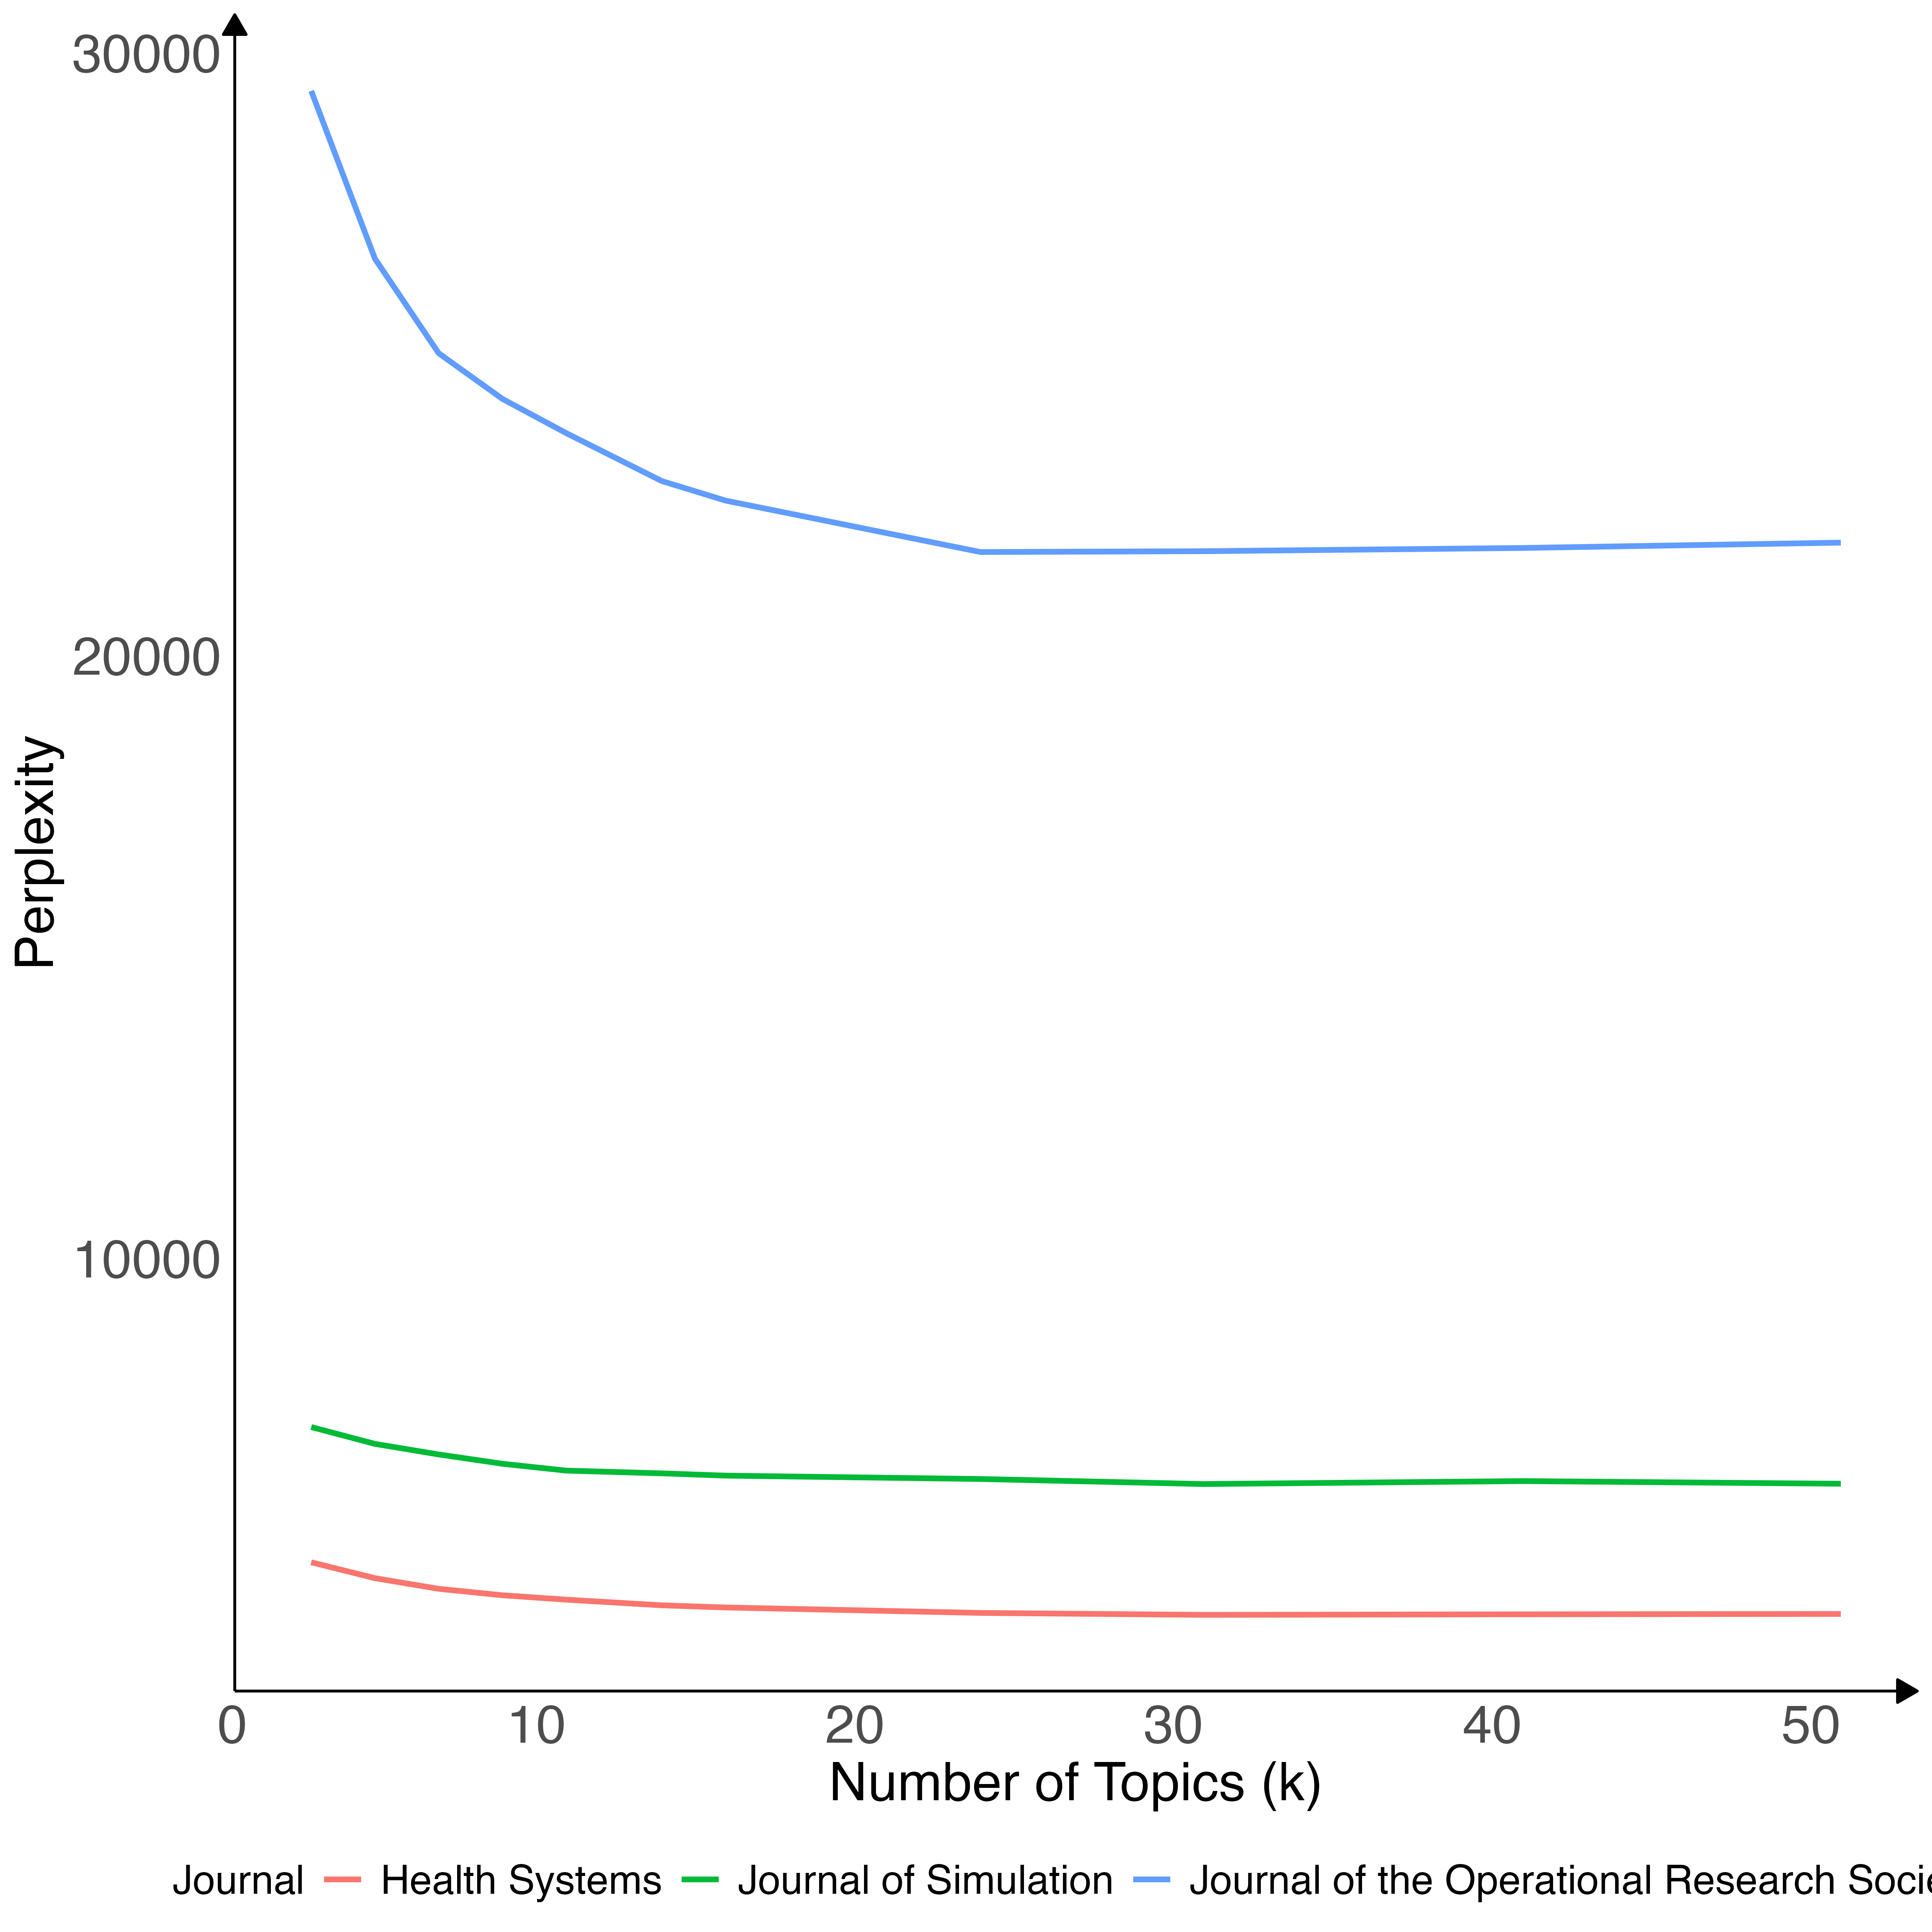
\includegraphics[width=0.49\linewidth]{bag_words/Perplexity_journal.png}

\caption{The perplexity with different numbers of topics across years and journals.}
\label{fig:perplexity}
\end{figure}

\subsection*{Structural Topic Modelling} \

Structural Topic Modelling (STM)~\cite{10.4108/eai.13-7-2018.159623} provided a method to incorporate document-level metadata (e.g., publication year, journal name) into the topic modelling process, which builds on the foundation of LDA.  Several metrics can be used to evaluate the optimal $k$~\cite{stm}, such as \textit{Exclusivity}, \textit{Heldout Likelihood}, \textit{Residuals}, and \textit{Semantic Coherence} as shown in Table~\ref{tab:stm_metrics}.


\begin{table}[!htbp]
\centering
\caption{Comparison of STM Metrics for Different K Values}
\begin{tabular}{cccccc}
\toprule
\textbf{K} & \textbf{Exclus} & \textbf{Semcoh} & \textbf{Heldout} & \textbf{Residual} \\
\midrule
2  & 7.93 & -165.02 & -8.90 & 61.93 \\
4  & 8.82 & -184.20 & -8.92 & 47.10 \\
6  & 9.41 & -236.94 & -8.97 & 36.15 \\
8  & 9.53 & -230.01 & -8.94 & 29.66 \\
10 & 9.67 & -219.33 & -8.86 & 24.15 \\
12 & 9.76 & -219.71 & -8.84 & 19.81 \\
14 & 9.76 & -216.37 & -8.81 & 16.59 \\
16 & 9.80 & -223.70 & -8.88 & 14.75 \\
18 & 9.79 & -213.05 & -8.84 & 12.42 \\
20 & 9.73 & -223.25 & -8.98 & 11.30 \\
\bottomrule
\end{tabular}
\label{tab:stm_metrics}
\end{table}

The STM metrics suggest that $k = 10$ is a reasonable choice, as the majority of the metrics remain stable at this point compared to the stable case of $k = 20$ using LDA shown in Figure~\ref{fig:perplexity}.


\begin{figure}[!tbhp]
\centering
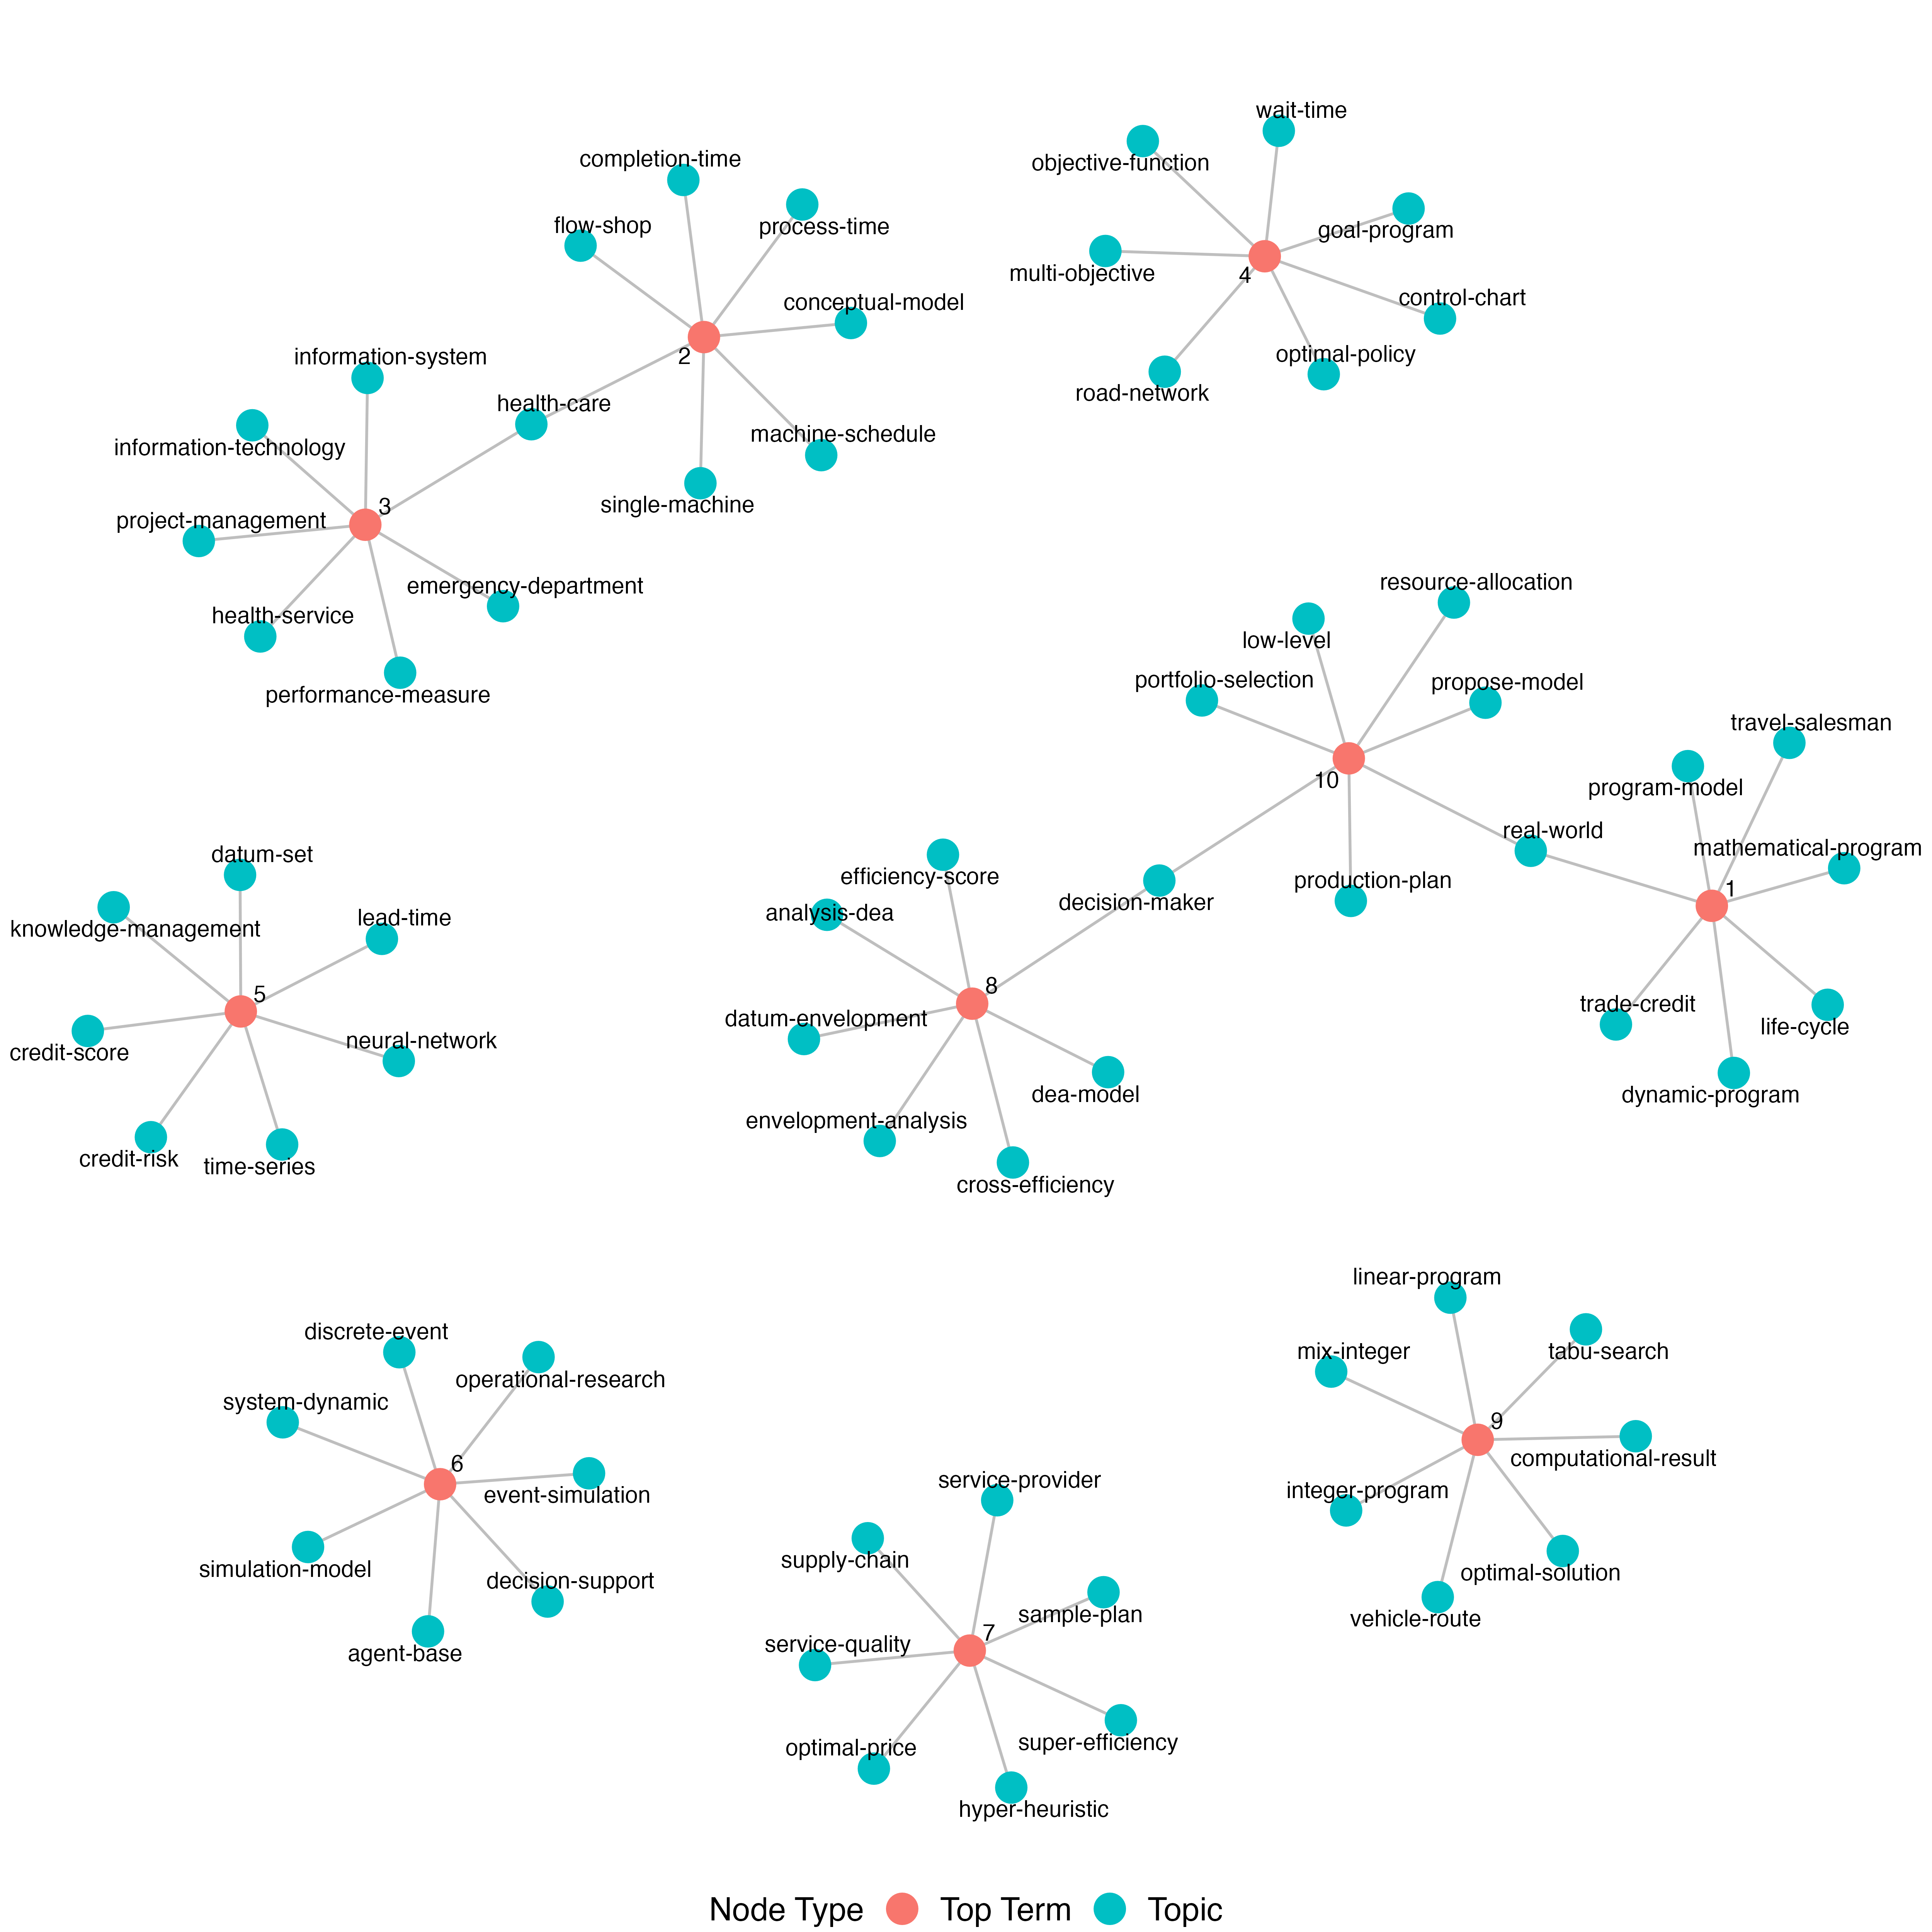
\includegraphics[width=0.7\linewidth]{bag_words/topics_STM10.png}
\caption{The identified topics using STM with the number of topics $k = 10$.}
\label{fig:stmtopics}
\end{figure}

The similarity $S$ of topics $i$ and $j$ between two models can be evaluated by Formula~\ref{eqn:similarity}~\cite{HAN201239}:

\vspace*{-12pt}
\begin{align}
S_{ij} =\frac{\sum_{w=1}^n A_{wi} B_{wj}}{\sqrt{\sum_{w=1}^n A_{wi}^2} \times \sqrt{\sum_{w=1}^n B_{wj}^2}} \numberthis \label{eqn:similarity} 
\end{align}\vspace*{-12pt}

Where $A_{wi}$ and $B_{wj}$ are the probabilities $\beta_{wi}=P\left(\operatorname{word}_w \mid \operatorname{topic}_i\right)$ and $\beta_{wj}=P\left(\operatorname{word}_w \mid \operatorname{topic}_j\right)$ of the $w^{th}$ word from the LDA model and STM model.

The similarity matrix shown in Figure~\ref{fig:similarity} suggests that 50\% of topics have a similarity greater than 0.7, and 80\% of topics have a similarity greater than 0.4 between the two models with the same number of topics $k=10$.

\begin{figure}[!tbhp]
\centering
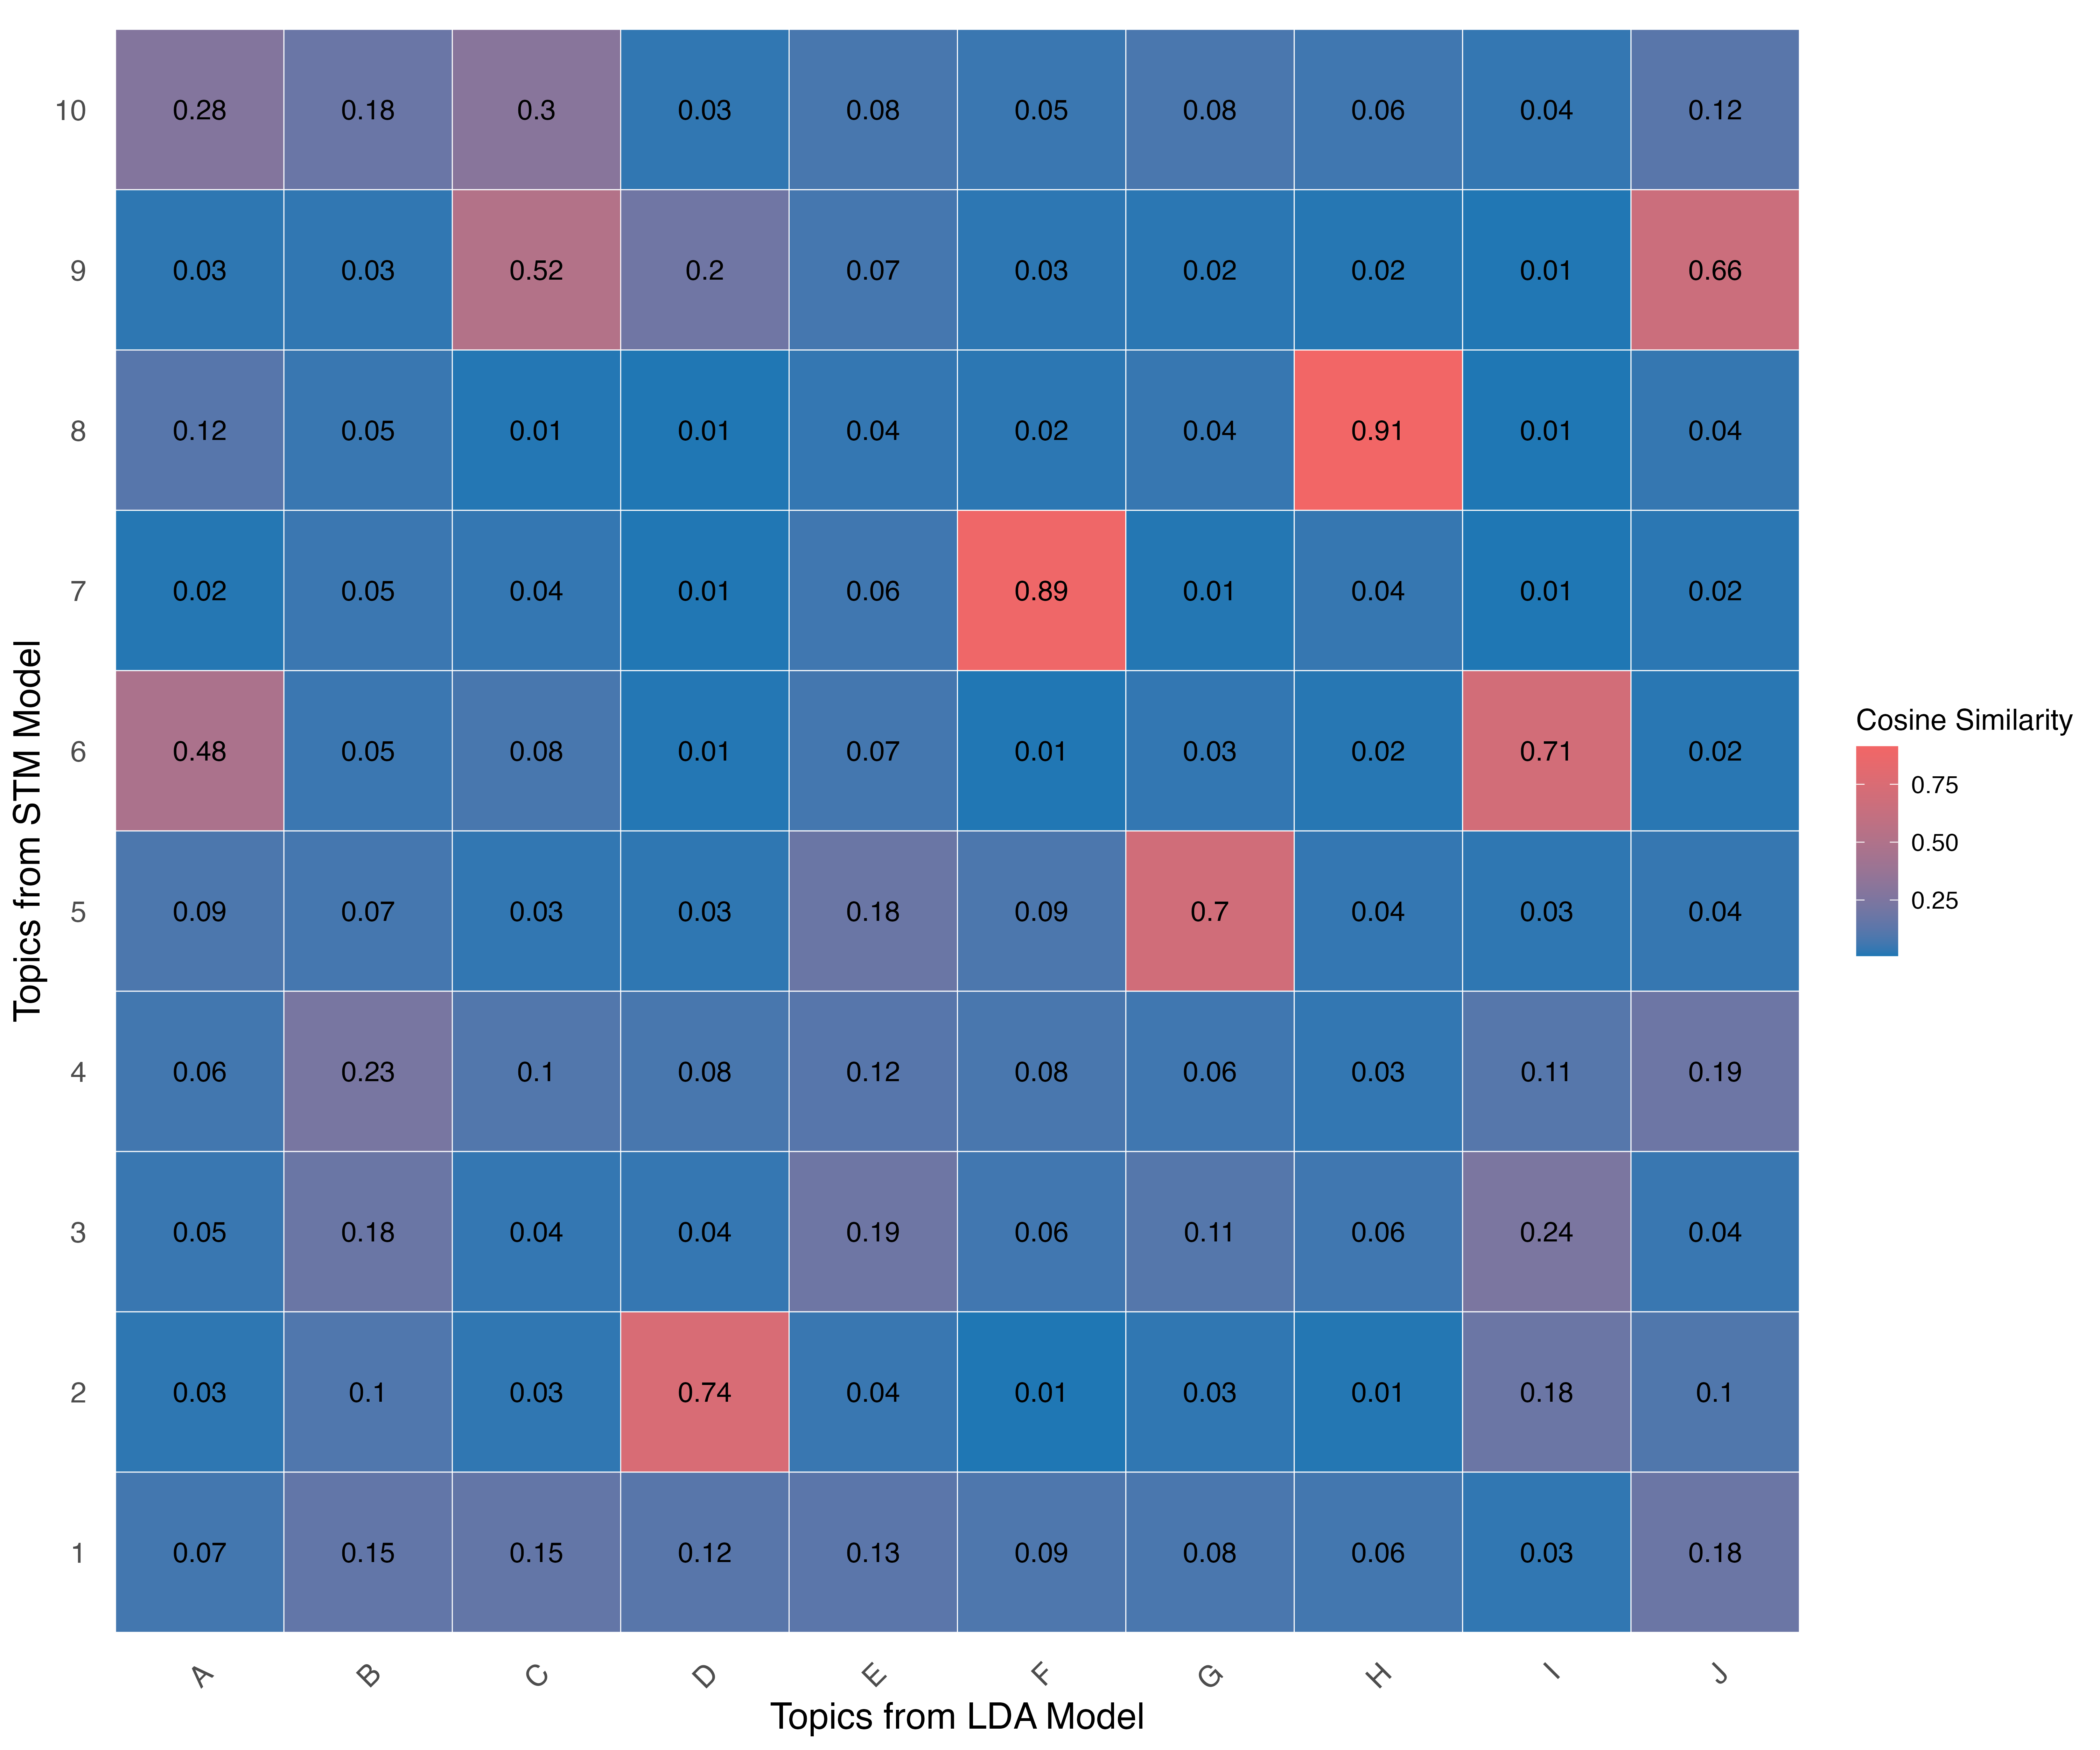
\includegraphics[width=0.6\linewidth]{bag_words/simularity_matrix.png}
\caption{The similarity matrix between LDA and STM models with topic number $k = 10$.}
\label{fig:similarity}
\end{figure}

One of the benefits of the STM model is that it can easily reveal the topic trend with data features like time. As shown in Figure~\ref{fig:STMtrend}, topics 1, 10, 7, and 8 demonstrate an increasing trend in popularity over the years. In contrast, topics 2, 3, 4, and 5 suggest a potential decline in popularity, although with wide uncertainty bands. Notably, topics 6 and 9 show clear and consistent decreases in popularity over time.

\begin{figure}[!tbhp]
\centering
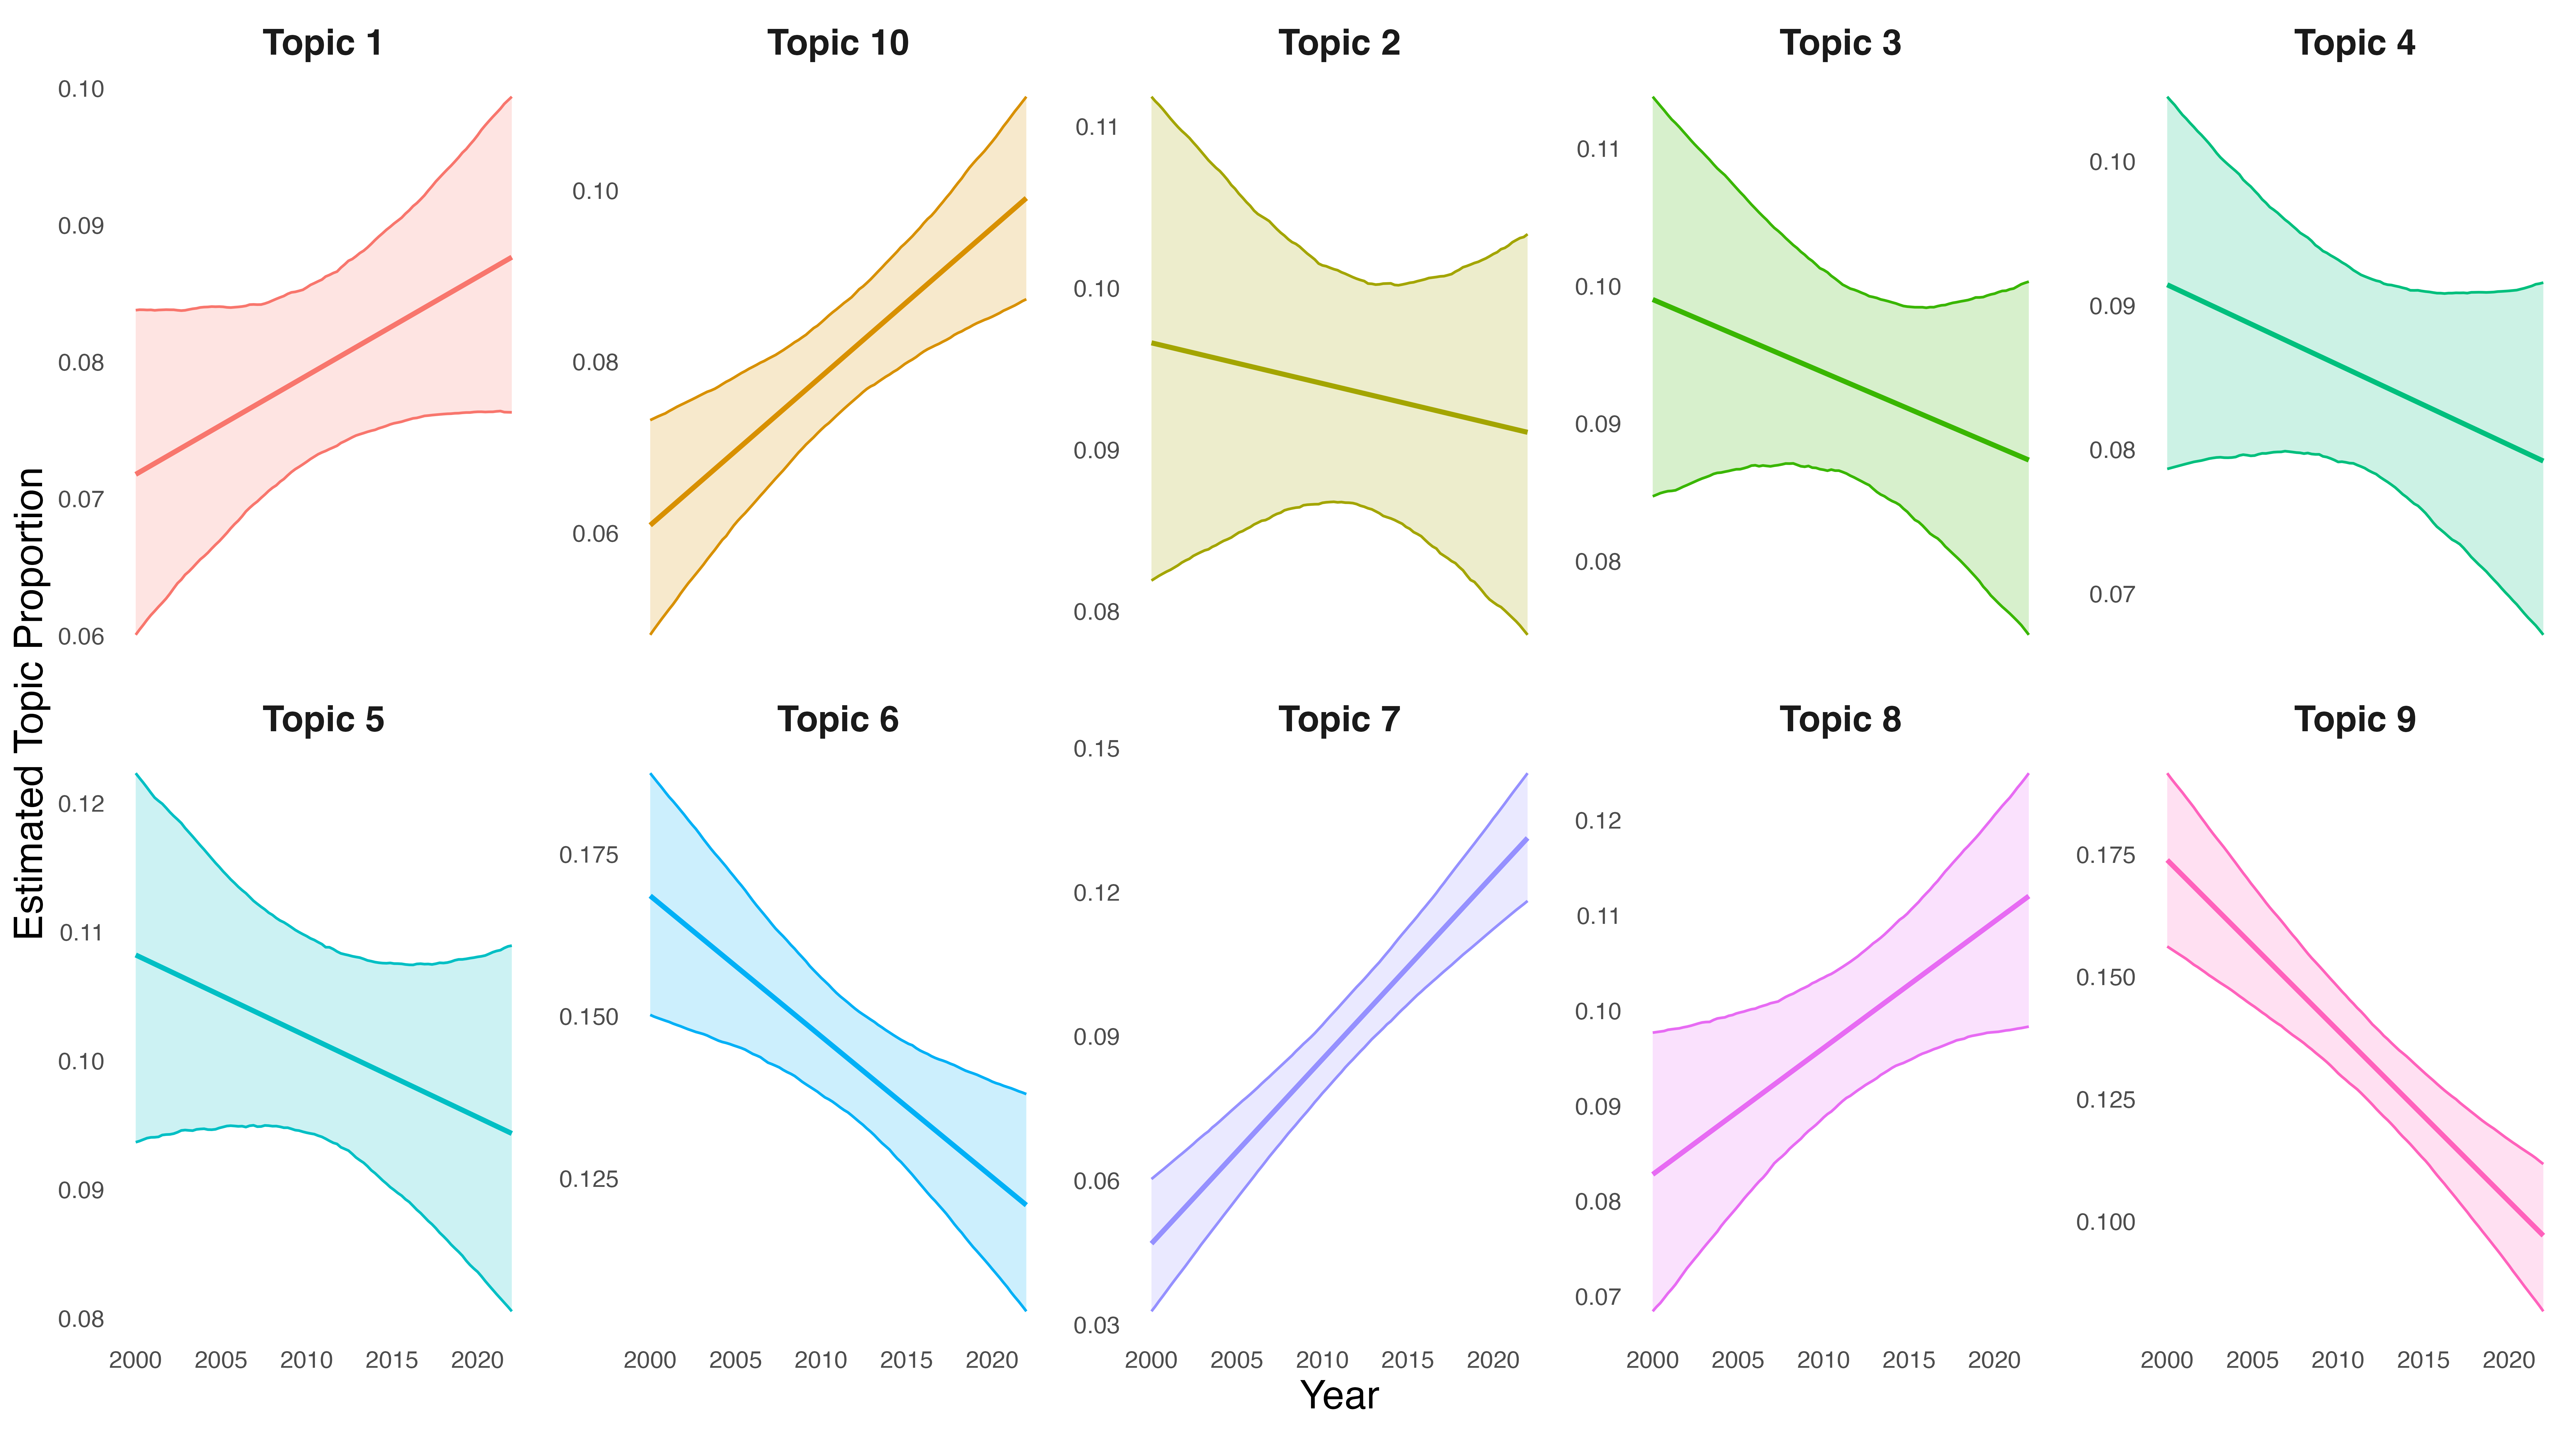
\includegraphics[width=0.9\linewidth]{bag_words/STM_trendtime.png}
\caption{Topic trends over time with the STM model and topic number $k = 10$.}
\label{fig:STMtrend}
\end{figure}

\section*{Citations Prediction with Regression}

\subsection*{Preprocessing} \

The topic probabilities generated by the two models were combined with the original data as features for regression analysis. The dataset was split into 80\% training data and 20\% test data to evaluate model performance. Additionally, the Journal Name column was transformed using one-hot encoding to convert categorical values into binary features.

The missing 'Views' values in the training data are filled using predictions from a linear regression model based on 'Citations,' while in the test data, they are replaced with mean values.

\subsection*{Linear Regression} \

Although two topic models, LDA and STM, have been trained, the similarity may lead to redundancy in the features generated from both models with the same $k$ value. The redundancy can negatively affect regression models~\cite{lm} due to multicollinearity. Principal Component Analysis (PCA)~\cite{doi:10.1080/14786440109462720} is applied to reduce the dimensionality of the combined topic distributions and transform correlated features into a set of uncorrelated principal components. As shown in Figure~\ref{fig:lmpca}, the first 23 PCA components are selected to train the linear regression model.


\begin{figure}[!tbhp]
\centering
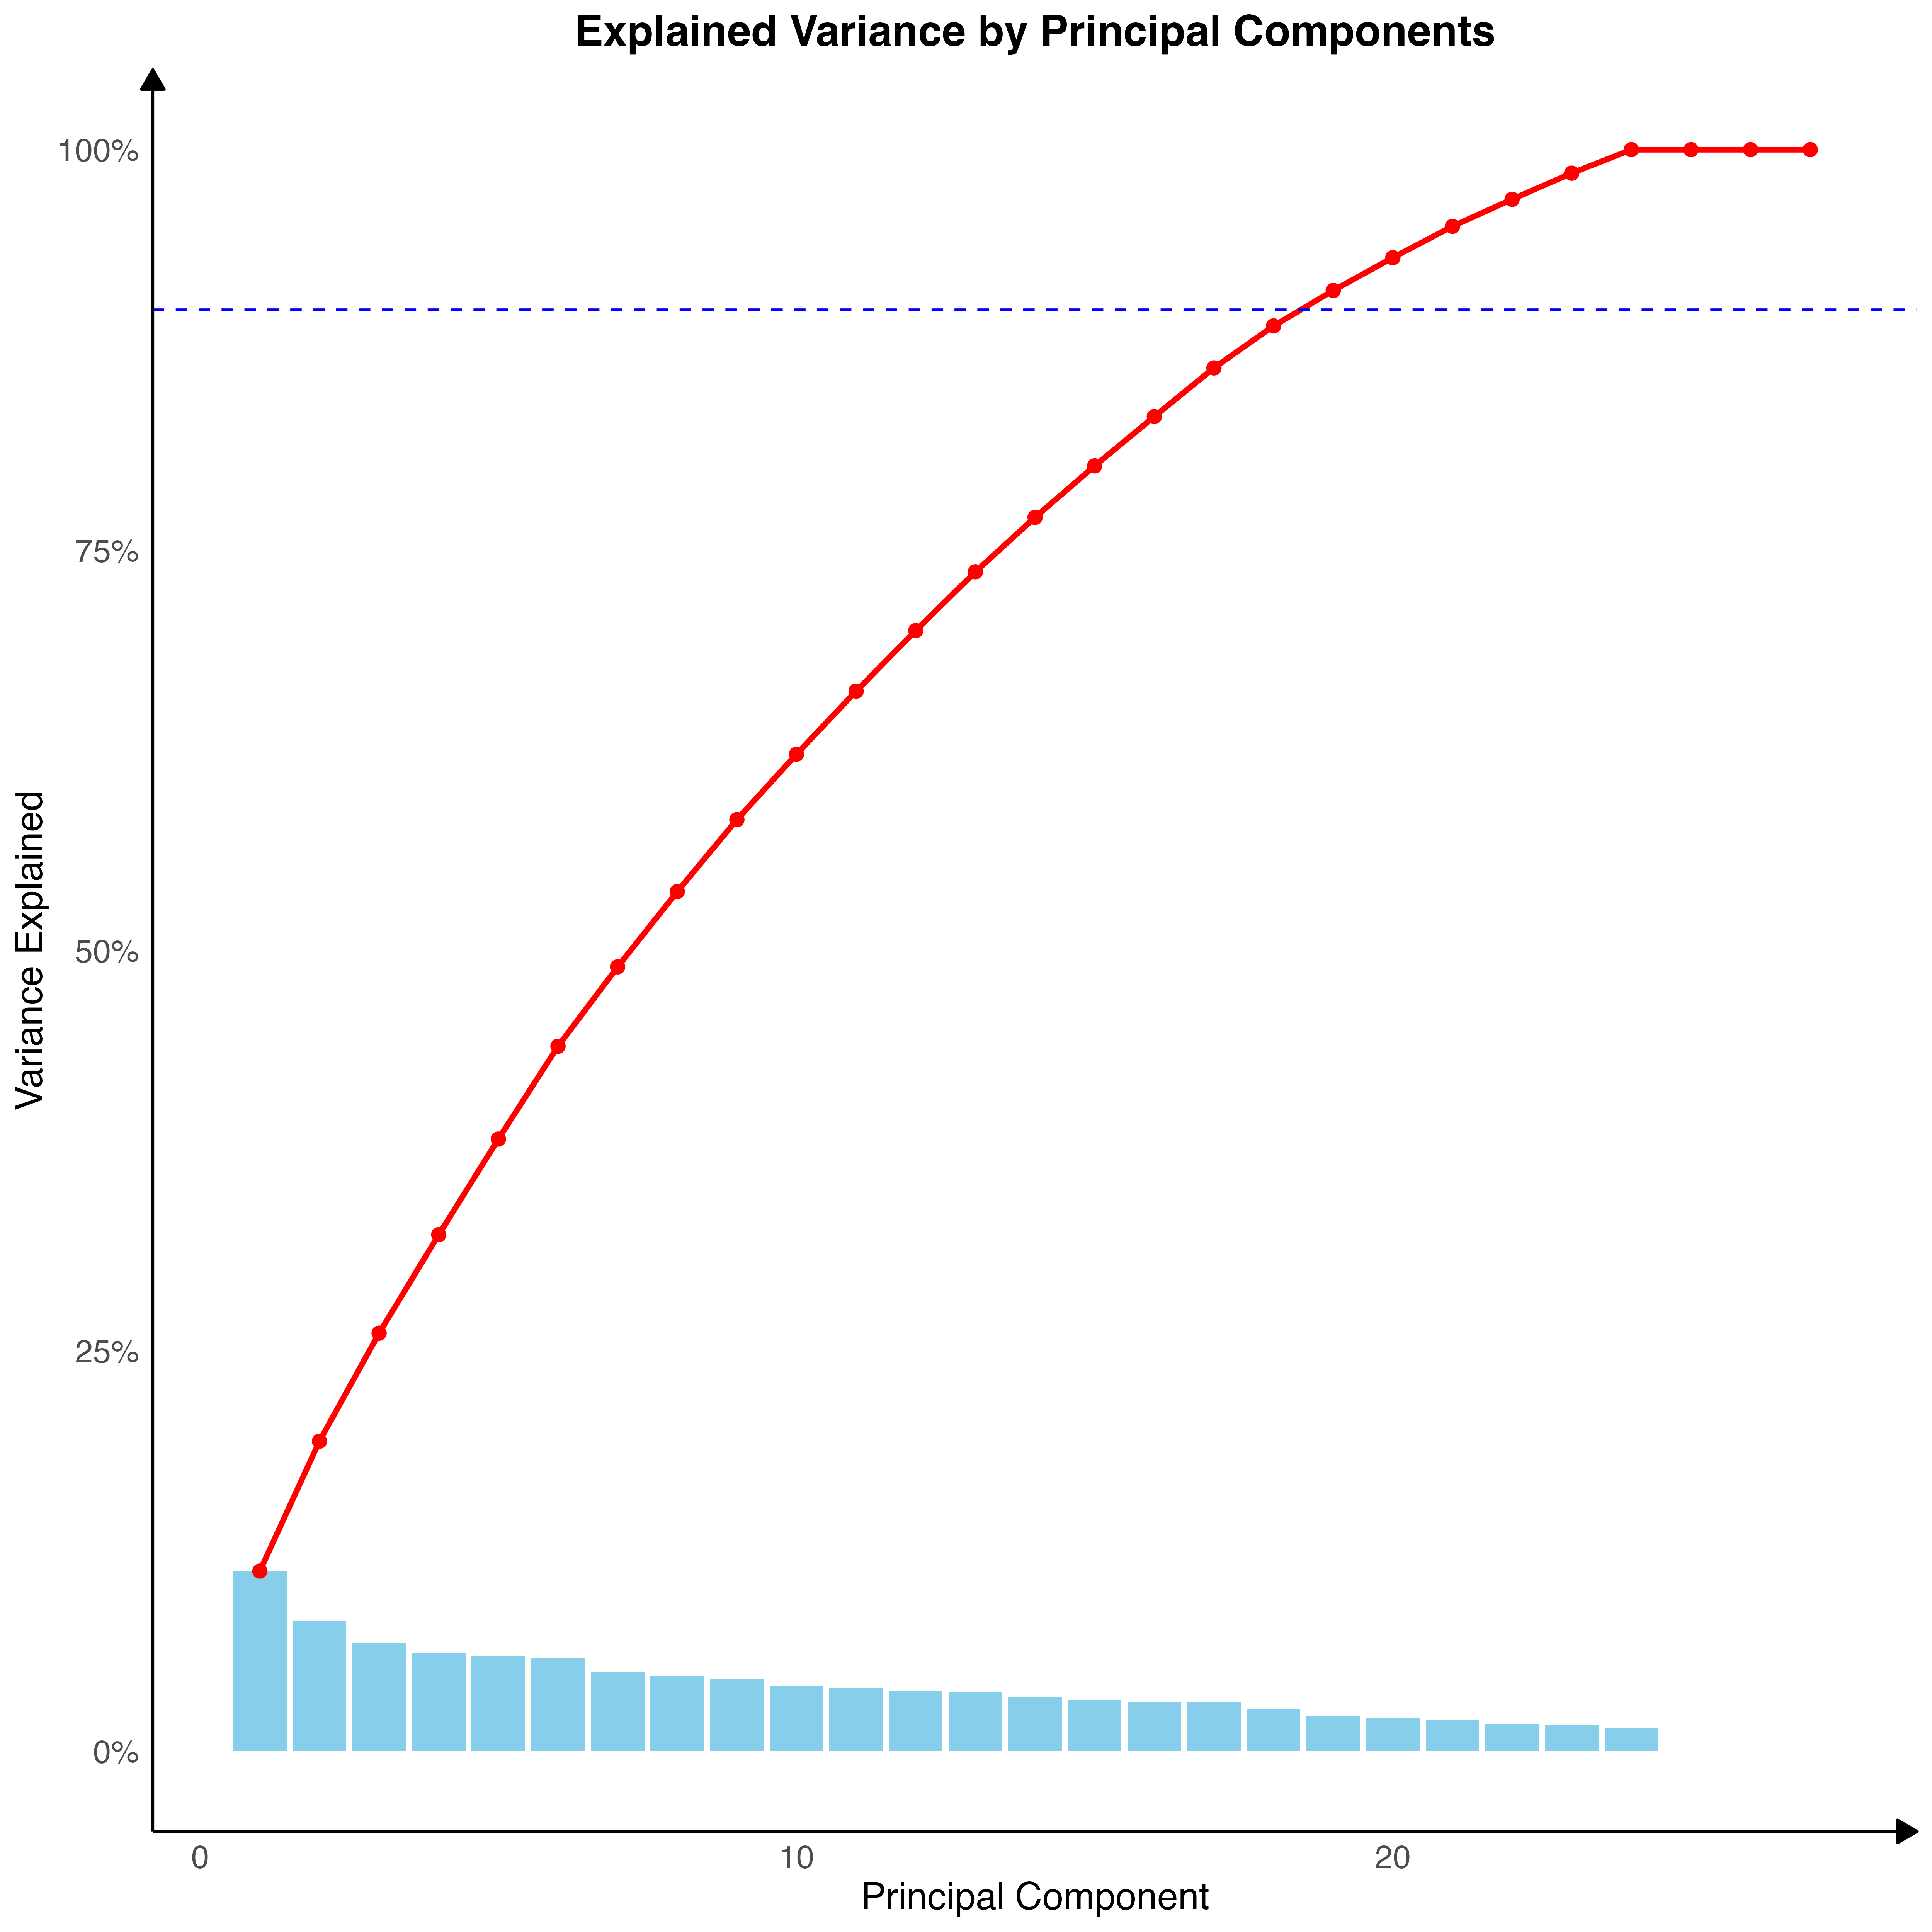
\includegraphics[width=0.5\linewidth]
{regression/pca_regression_lm.png}
\caption{Explained and cumulative variances by principal components.}
\label{fig:lmpca}
\end{figure}


\subsection*{XGBoost}
eXtreme Gradient Boosting (XGBoost)~\cite{10.1145/2939672.2939785} uses gradient boosting, minimising a loss function by adding new trees that predict the residual errors of the previous trees. However, the effectiveness of this process heavily depends on the selection of appropriate hyperparameters. In this work, a grid search is applied, as shown in Table~\ref{tab:grid_scan} for optimal choice.



\subsection*{RandomForest}

Compared to XGBoost, Random Forest~\cite{Breiman2001} takes a different approach by employing an ensemble of independent decision trees.  Similar to XGBoost, the performance of Random Forest is sensitive to hyperparameter selection. A grid search is similarly conducted, as shown in Table~\ref{tab:grid_scan}, to identify the best combination of hyperparameters for Random Forest.



%Term frequency-inverse document frequency (TF-IDF) is also an important feature that can highlight the significance of specific terms within a document relative to a collection of documents. 
\begin{table}[ht]
\centering
\caption{The grid scan for XGBoost and Random Forest}
\resizebox{\linewidth}{!}{%
\begin{tabular}{c c c c}
\hline
\textbf{Model}        & \textbf{Parameter}       & \textbf{Description}    & \textbf{Scan range}                  \\
\hline
\multirow{7}{*}{XGBoost}  & nrounds                & Number of boosting rounds      & 100, 300, 500             \\
                         & $\eta$                  & Learning rate                  & 0.005, 0.01, 0.03, 0.1    \\
                         & max\_depth              & Maximum depth of trees         & 5, 8, 10                  \\
                         & $\gamma$                & Minimum loss reduction         & 0, 1                      \\
                         & colsample\_bytree       & Column subsample ratio         & 0.8, 1.0                  \\
                         & min\_child\_weight      & Minimum sum of instance weight & 1, 5, 10                  \\
                         & subsample               & Row subsample ratio            & 0.8, 1.0                  \\
\hline
\multirow{3}{*}{Random Forest} & mtry              & Number of variables tried at each split & 2, 5, 10        \\
                               & splitrule         & Splitting rule                & "variance", "extratrees"   \\
                               & min.node.size     & Minimum size of terminal nodes & 1, 5, 10        \\
\hline
\end{tabular}
}
\label{tab:grid_scan}
\end{table}

The three models are evaluated using four metrics: Mean Squared Error (MSE), Root Mean Squared Error (RMSE), Coefficient of Determination ($\text{R}^2$), and Residuals, as shown in Figure~\ref{fig:metrics_res}. The linear regression model shows the poorest performance due to the non-linear relationships between the target variable and the predictors.


\begin{figure}[!tbhp]
\centering
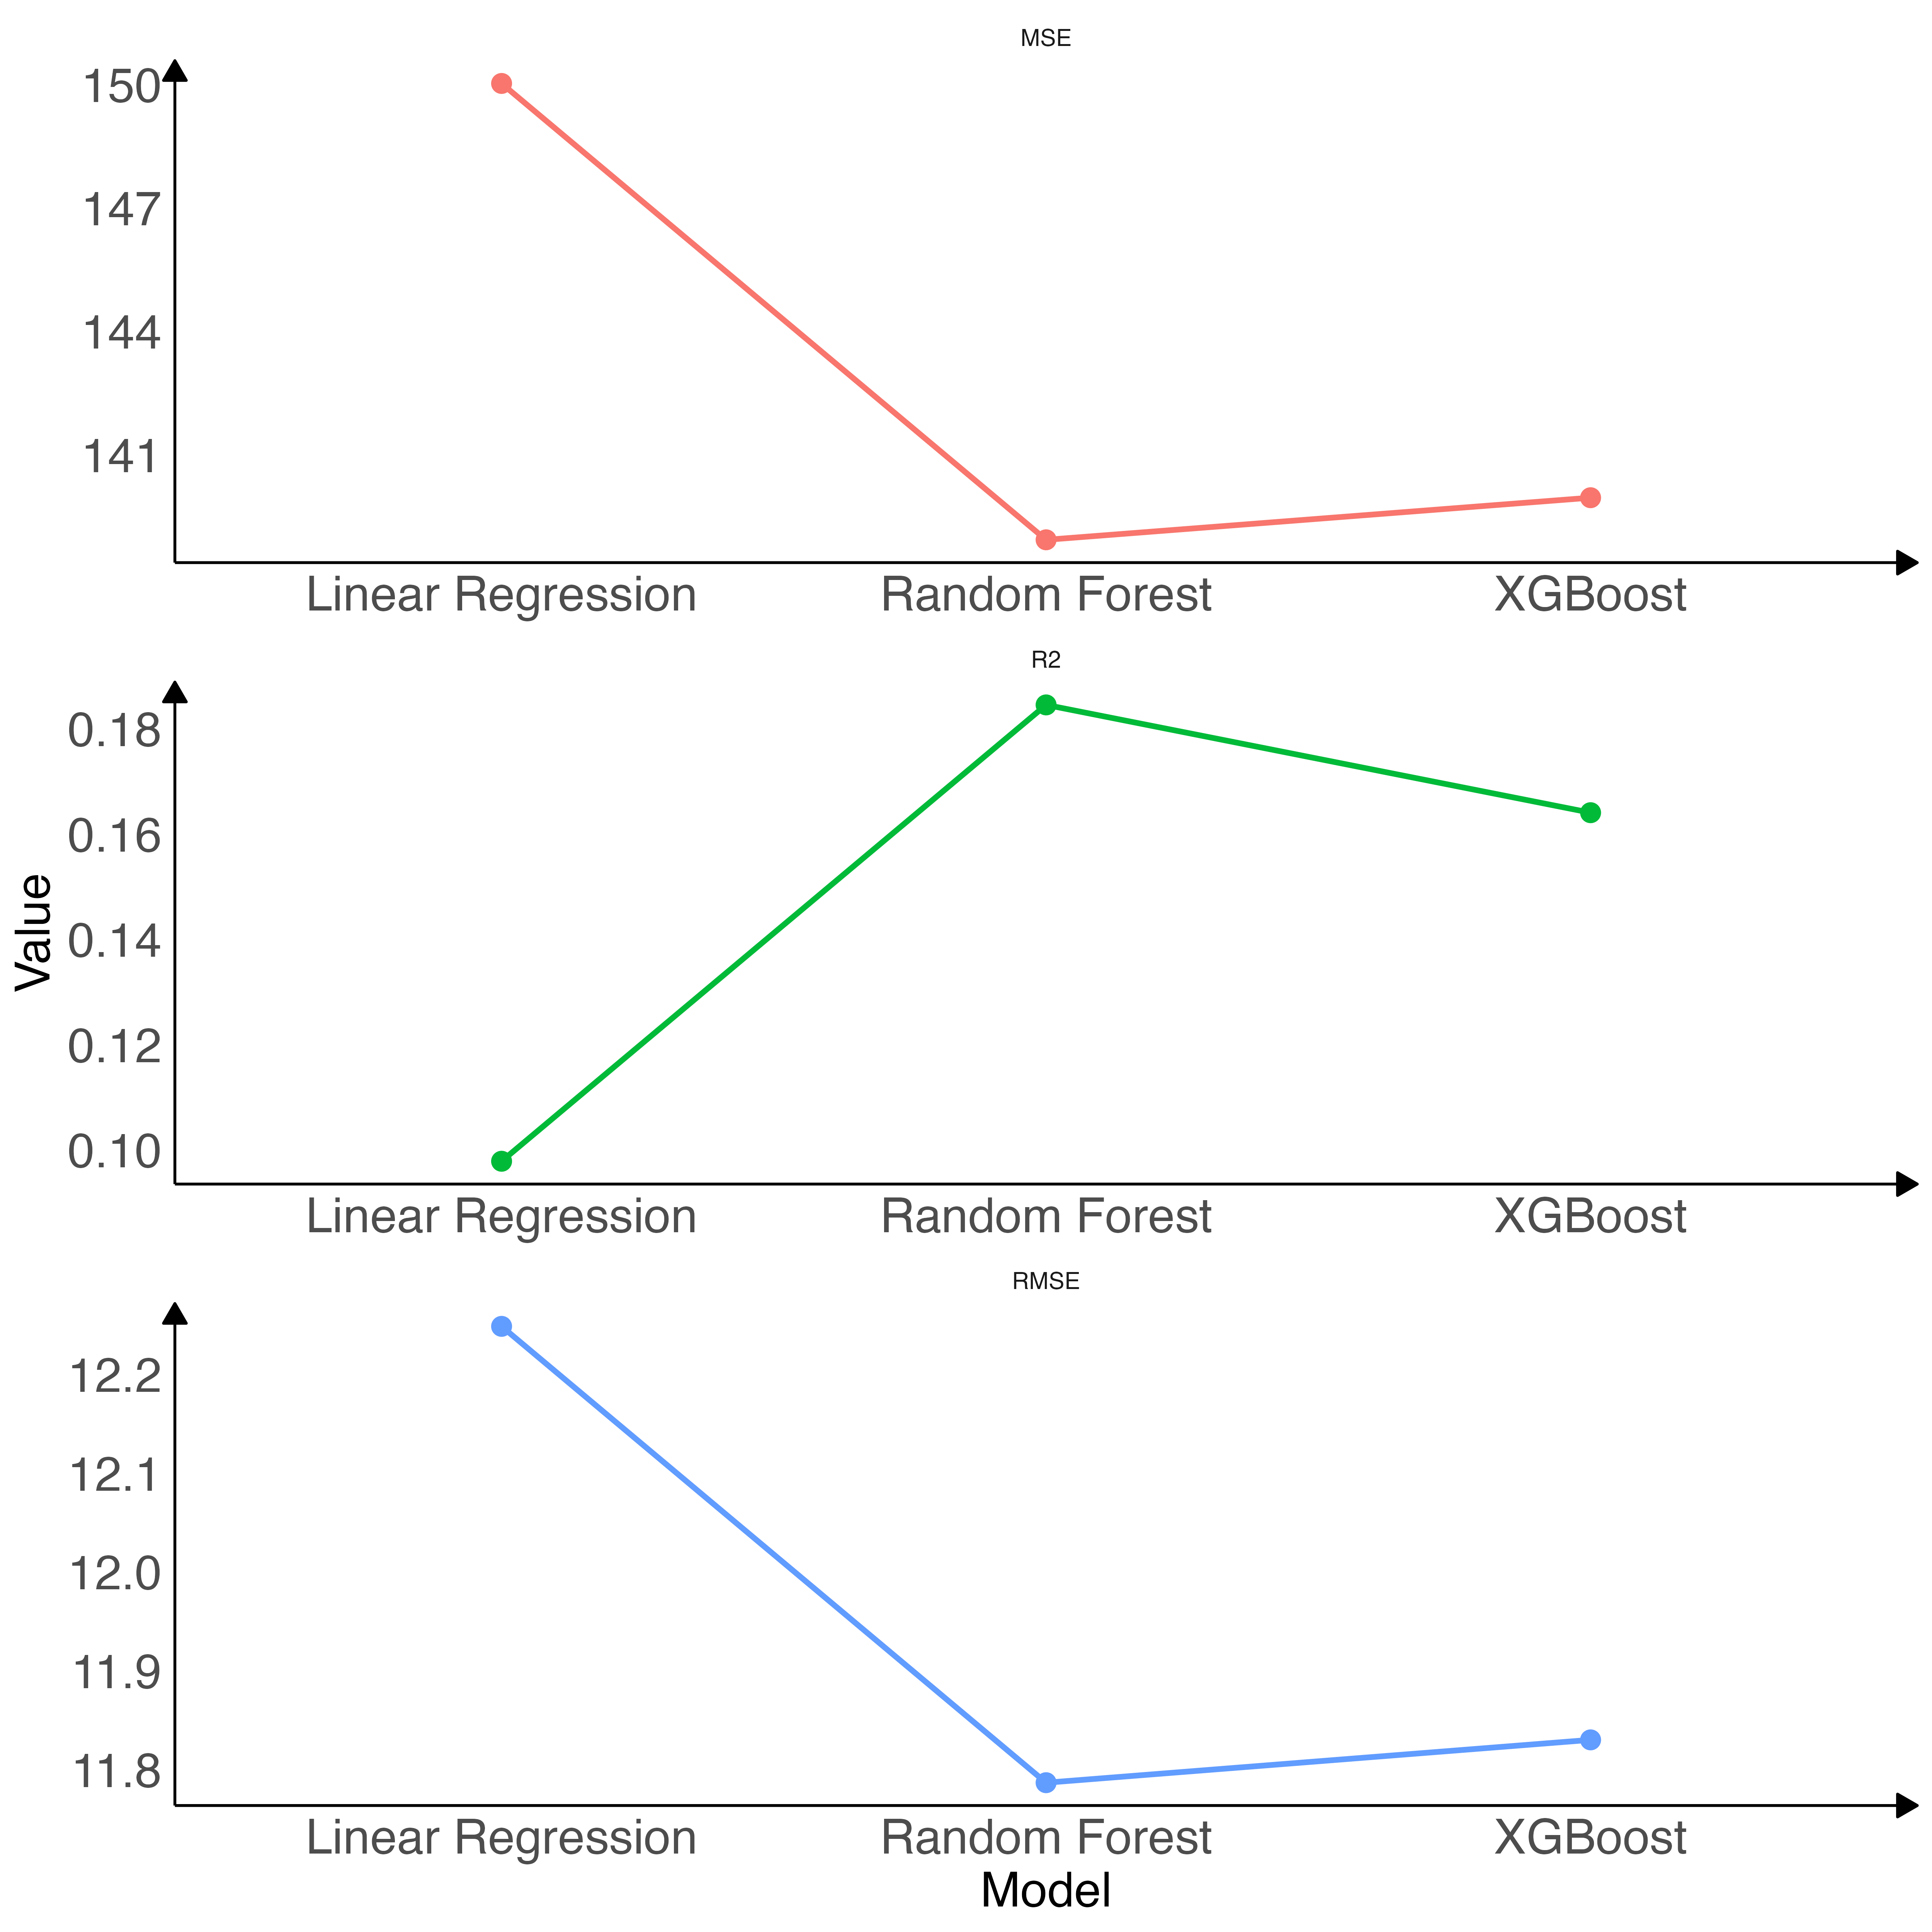
\includegraphics[width=0.4\linewidth]{regression/resgression.png}
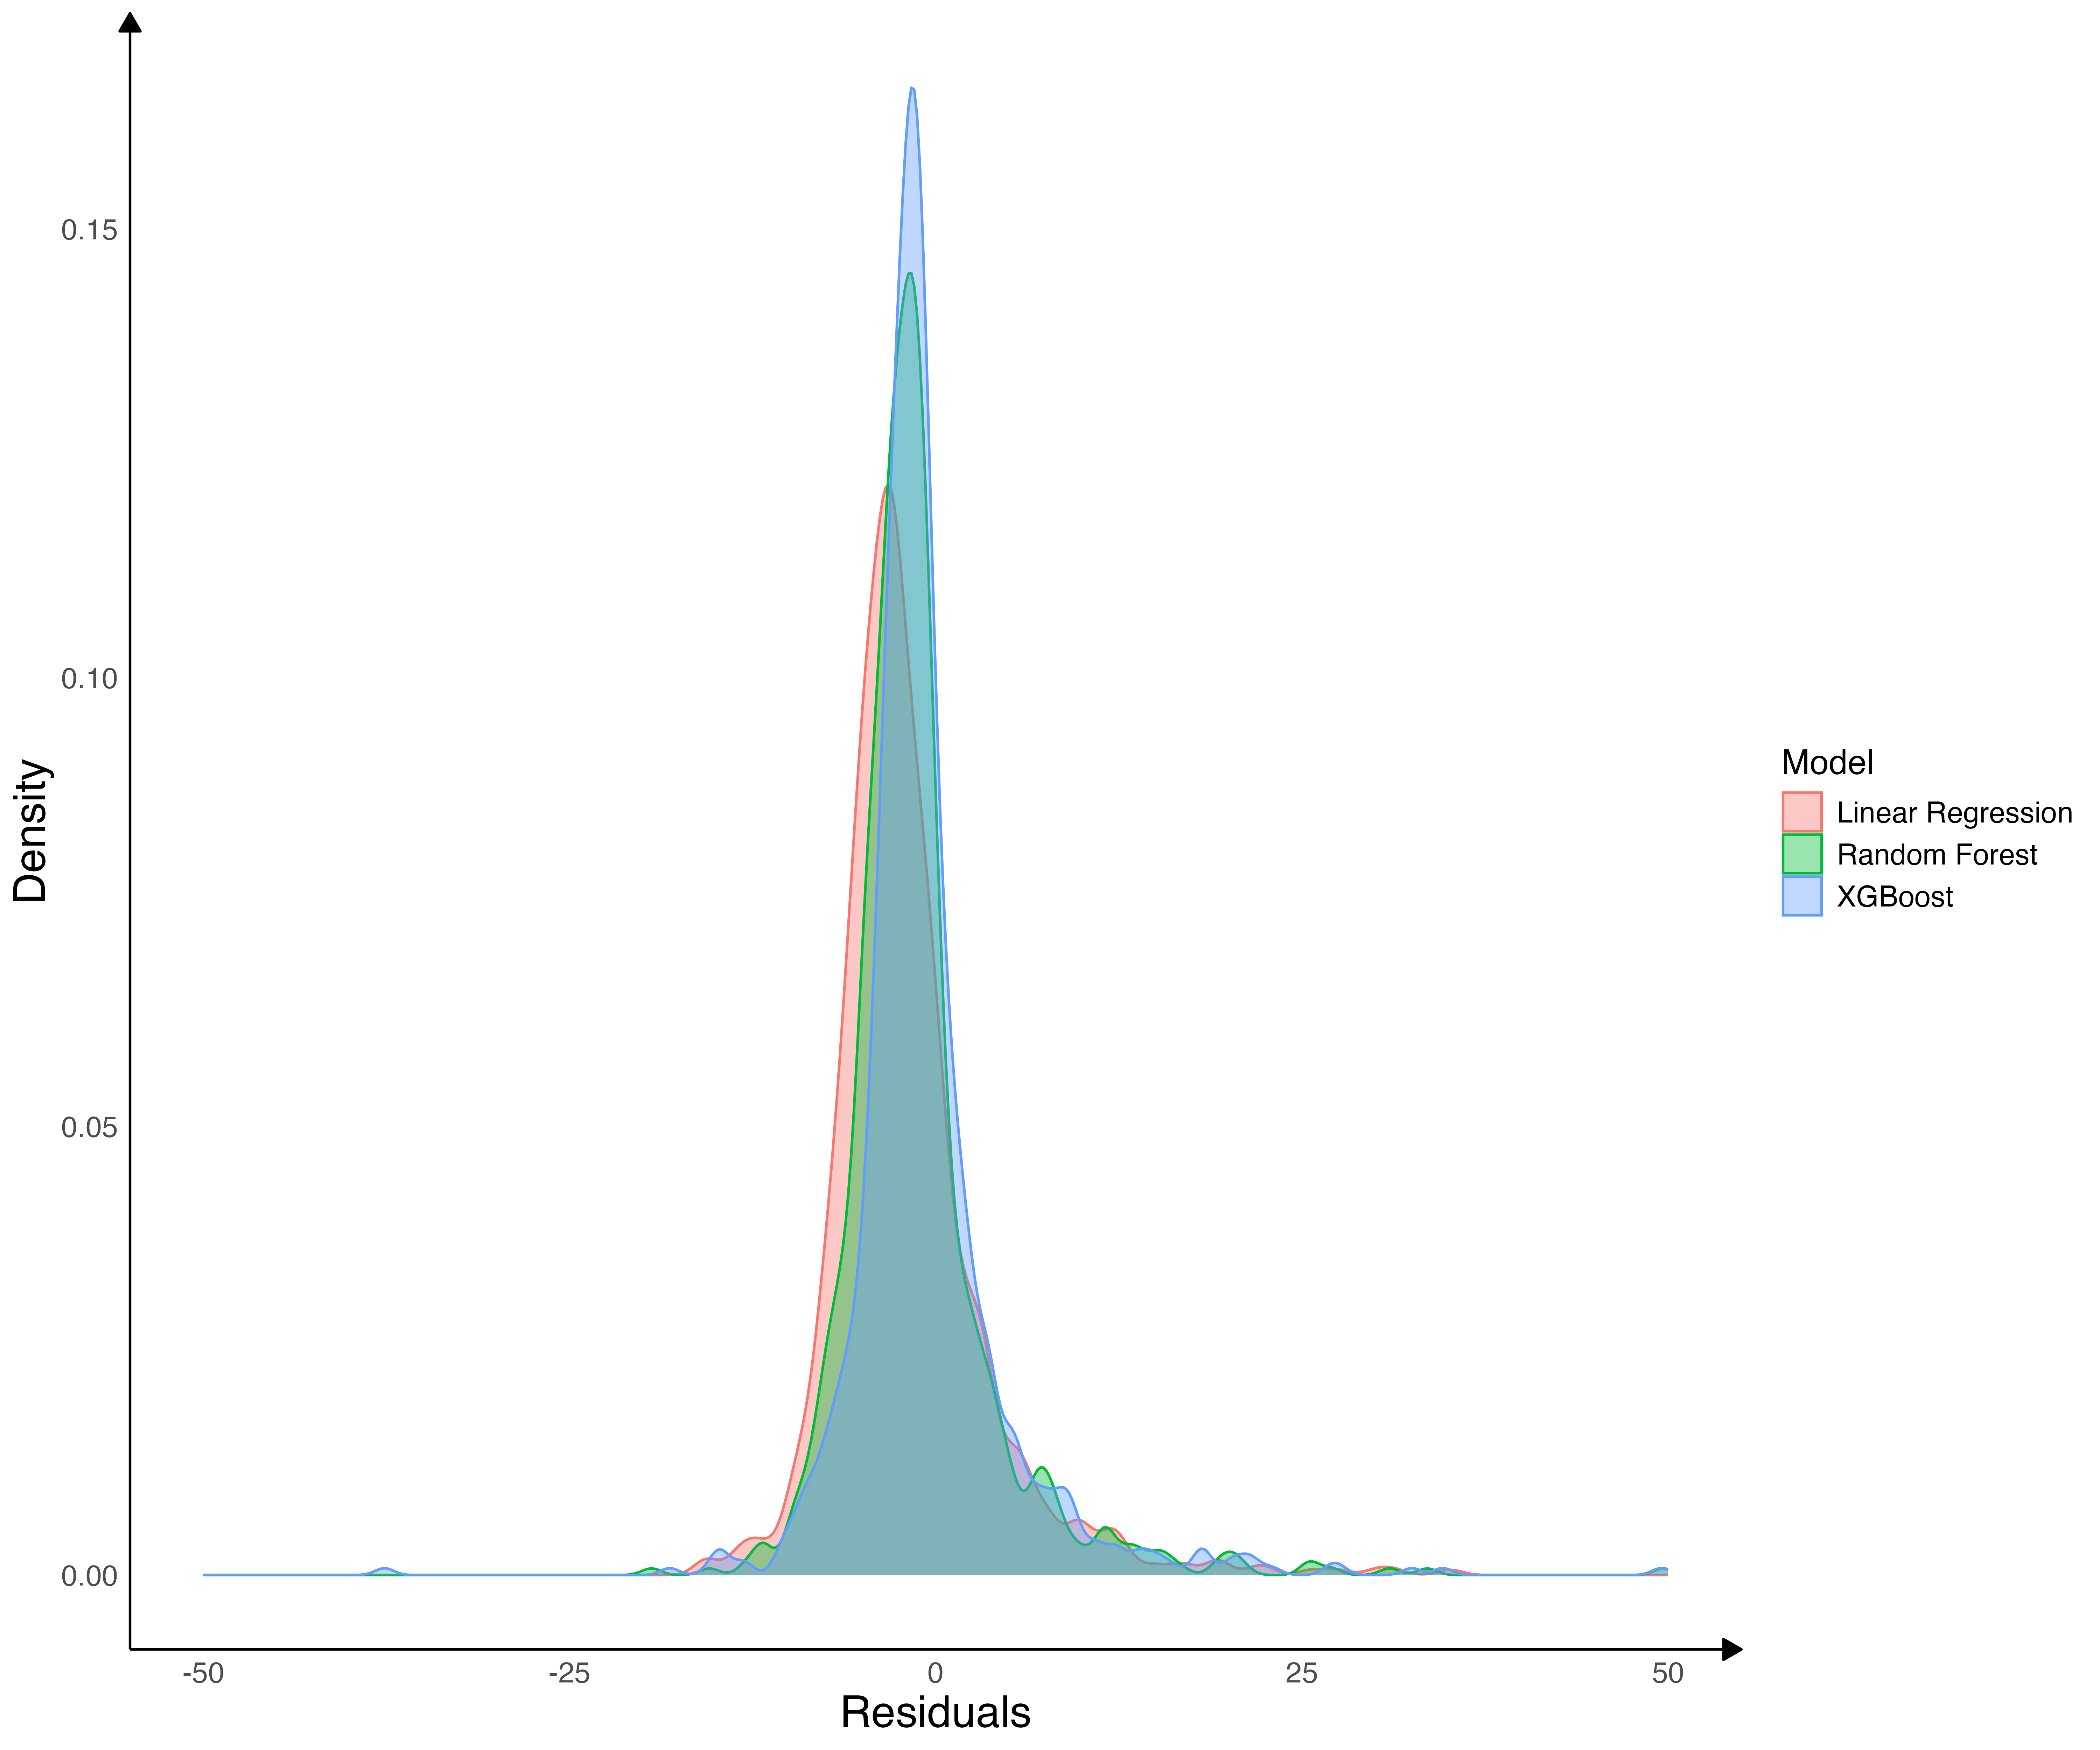
\includegraphics[width=0.58\linewidth]{regression/resgression_res.png}
\caption{MSE, RMSE, $\text{R}^2$, and residual density for regression model evaluations.}
\label{fig:metrics_res}
\end{figure}


\section{Classification}

\subsection*{Clustering for more information} \

Clustering~\cite{cluster} helps capture hidden patterns or latent groupings in the data that are not immediately obvious from the original features. These patterns can provide useful additional information for classification models to make better predictions.

In this work, a combined clustering approach is applied. The Hierarchical Density-Based Spatial Clustering of Applications with Noise (HDBSCAN) model~\cite{10.1145/2733381} is first used to generate initial clusters. The cluster labels obtained from HDBSCAN are then used as an input feature for the KMeans method~\cite{Jin2010} to build a second clustering model. The top three words with the highest mean Term Frequency-Inverse Document Frequency (TF-IDF)~\cite{ref1} scores for each cluster are presented in Table~\ref{tab:top_words_tfidf}. Additionally, the corresponding journal names are displayed in Table~\ref{tab:journal_cluster_counts}, which shows that Cluster 3 is associated with the "Journal of the Operational Research Society," while Clusters 1 and 2 provide useful insights for the other two journals.

\begin{table}[h]
\centering
\caption{Top Words with Highest TF-IDF Scores by Cluster}
\begin{tabular}{ccc}
\hline
\textbf{Cluster} & \textbf{Word} & \textbf{TF-IDF Score} \\
\hline
1 & supply chain        & 0.0105 \\
1 & operational research & 0.0108 \\
1 & datum envelopment    & 0.0077 \\
2 & supply chain        & 0.0102 \\
2 & operational research & 0.0090 \\
2 & simulation model     & 0.0073 \\
3 & research society    & 0.0290 \\
3 & operational research & 0.0275 \\
3 & supply chain        & 0.0092 \\
\hline
\end{tabular}
\label{tab:top_words_tfidf}
\end{table}


\begin{table}[h]
\centering
\caption{Number of Articles by Journal and Cluster}
\resizebox{\linewidth}{!}{%
\begin{tabular}{cccc}
\hline
\textbf{Cluster} & \textbf{Health Systems Journal} & \textbf{Journal of Simulation} & \textbf{Journal of the Operational Research Society} \\
\hline
1 & 122 & 164 & 963 \\
2 & 86  & 217 & 1281 \\
3 & 0   & 23  & 1285 \\
\hline
\end{tabular}
}
\label{tab:journal_cluster_counts}
\end{table}


Before classification, the training data is created by selecting 80\% of the original dataset, combined with cluster labels, STM and LDA topic predictions, and a binary variable indicating whether the document contains journal-specific frequent bigrams, as shown in Figure~\ref{fig:bagwordsjournal}. 

\subsubsection*{K-Nearest Neighbours}

K-Nearest Neighbours (KNN)~\cite{Mucherino2009} is a non-parametric, distance-based algorithm commonly used for classification tasks. The class label of a test sample is determined by a majority vote among its 20 nearest neighbours from the training data. The Euclidean distance metric was used to measure the similarity between samples.


\subsubsection*{Multinomial Logistic Regression}

Multinomial Logistic Regression (LG)~\cite{doi:https://doi.org/10.1002/9781119450382.ch10} is a supervised learning algorithm used for multi-class classification. The model predicts the class label by estimating the probability of each possible class. In this study, the predictions were trained by selecting the class with the highest probability for each test sample.

\subsubsection*{Random Forest}

The Random Forest model used for classification was trained with 500 trees and 3 features randomly selected at each split.

\begin{figure}%[tbhp]
\centering
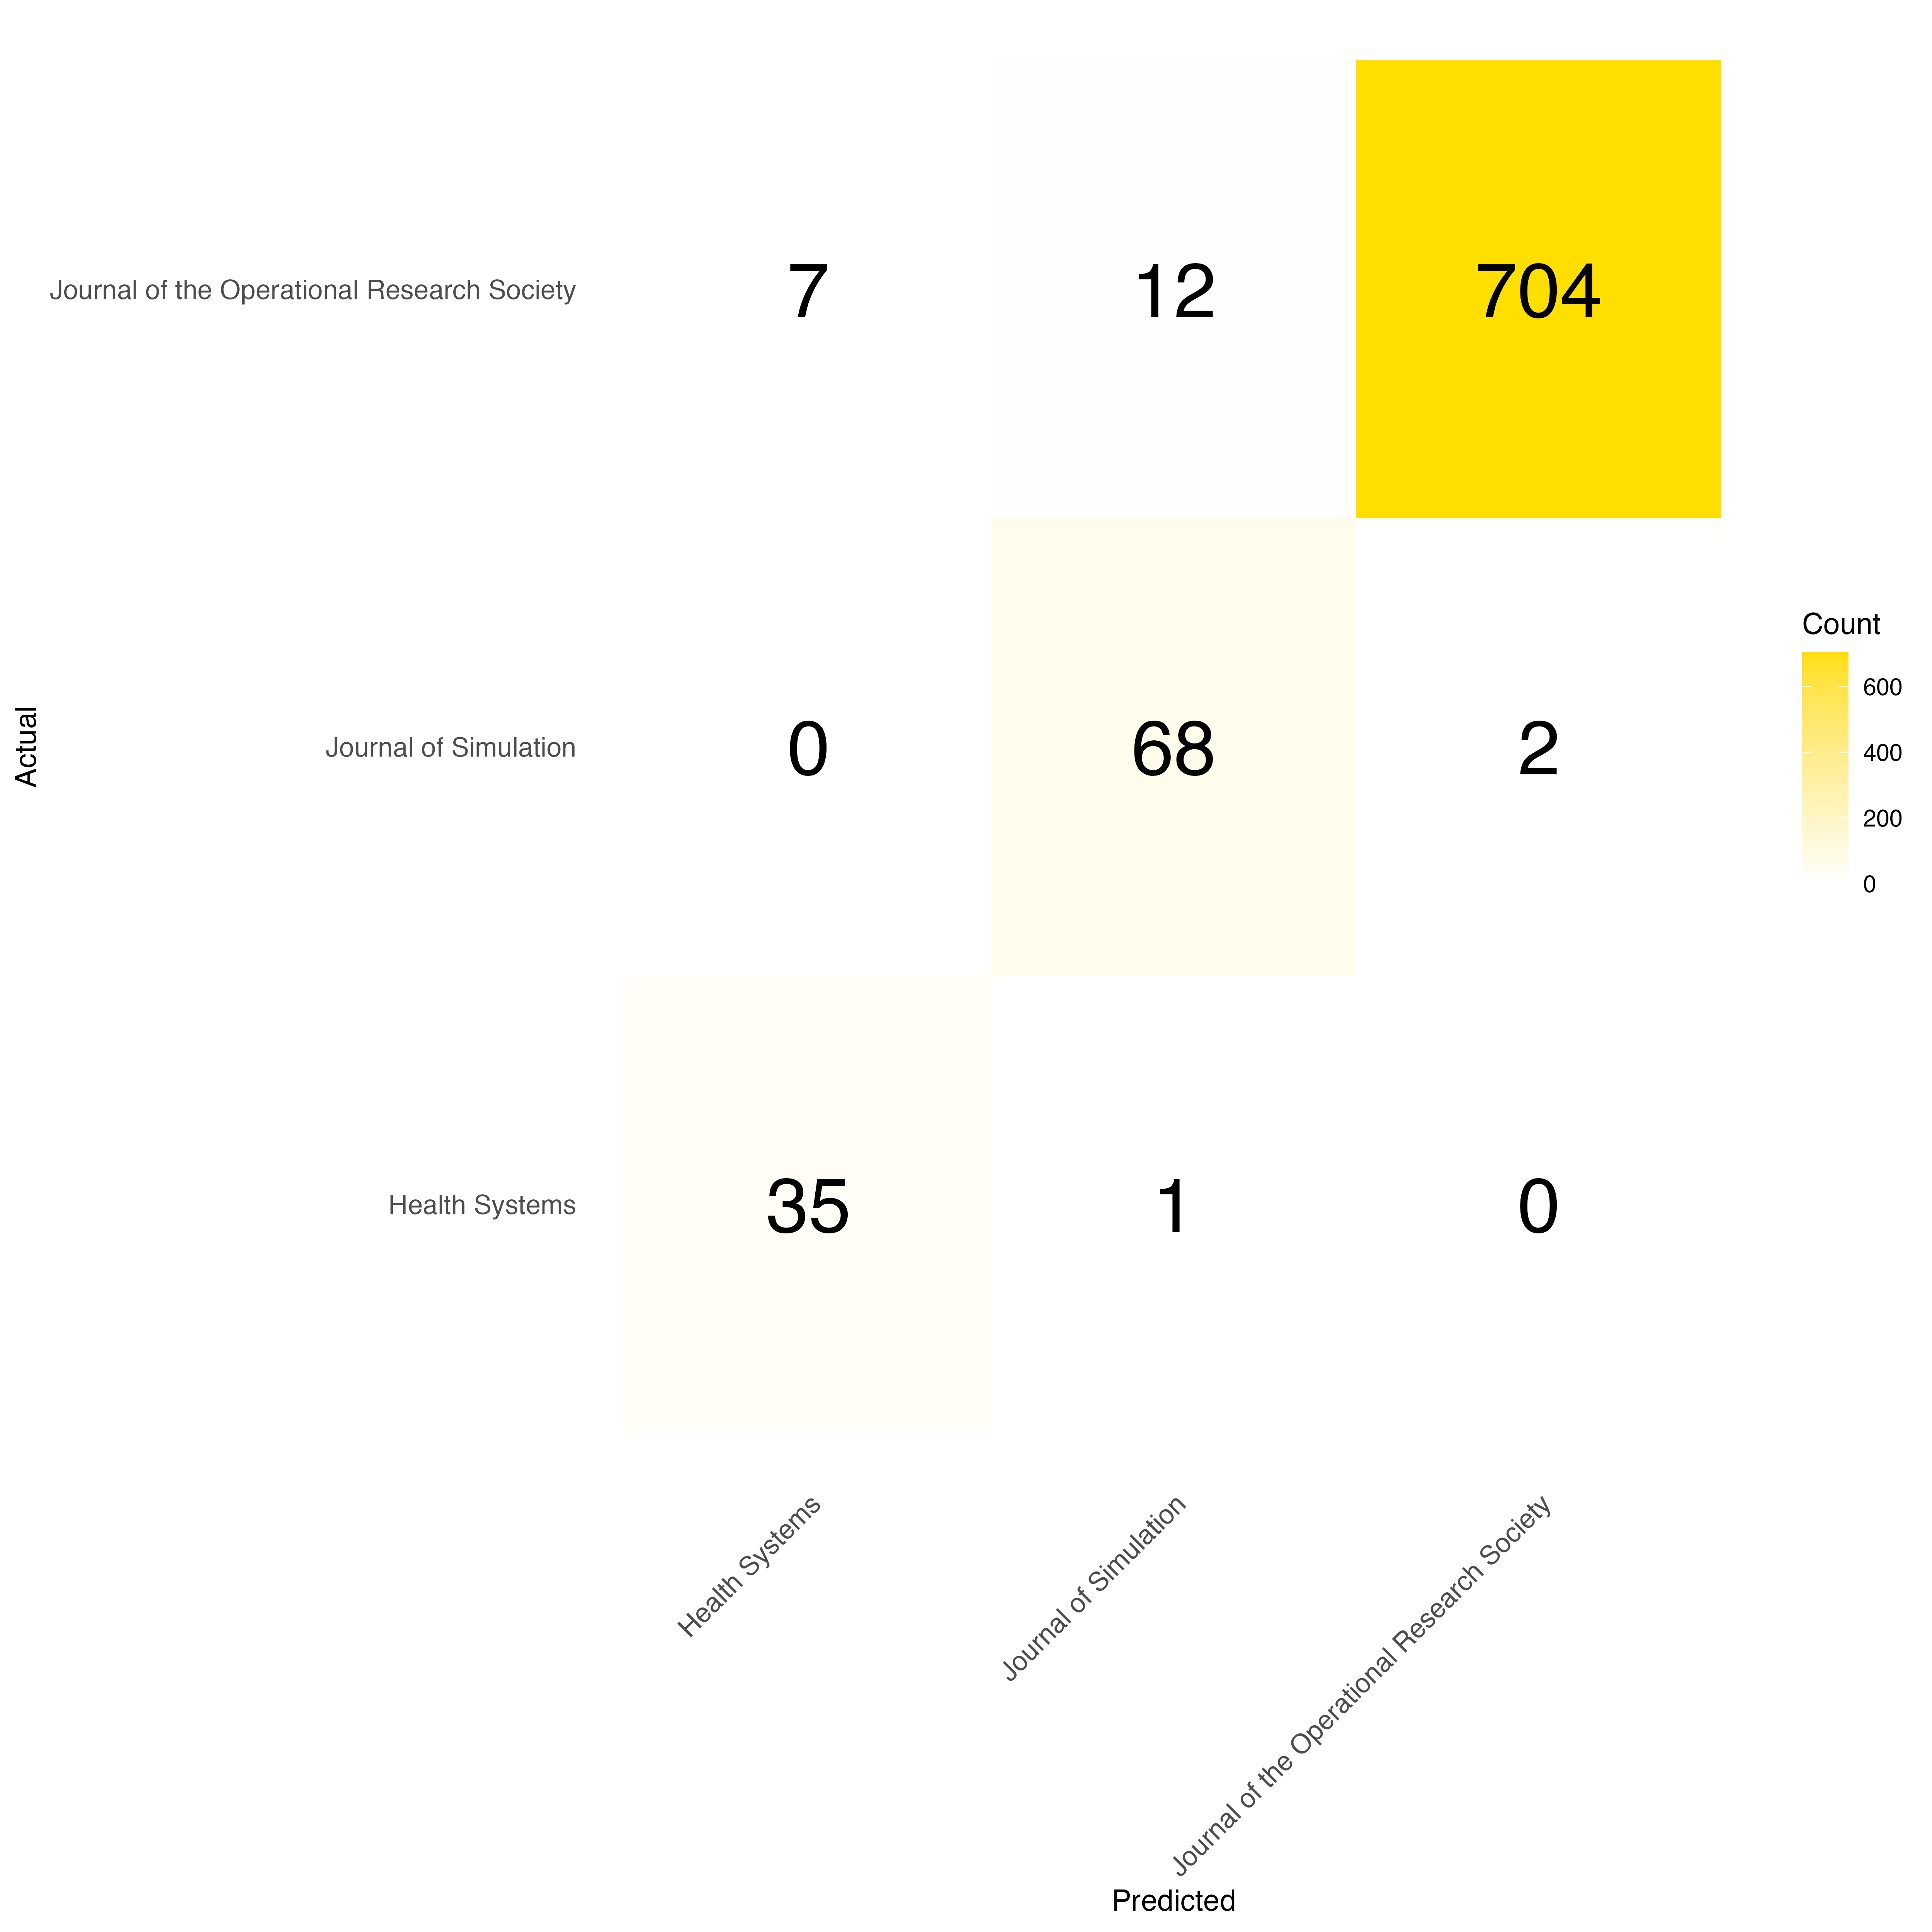
\includegraphics[width=.3\linewidth]{class/conf_RandomForest.png}
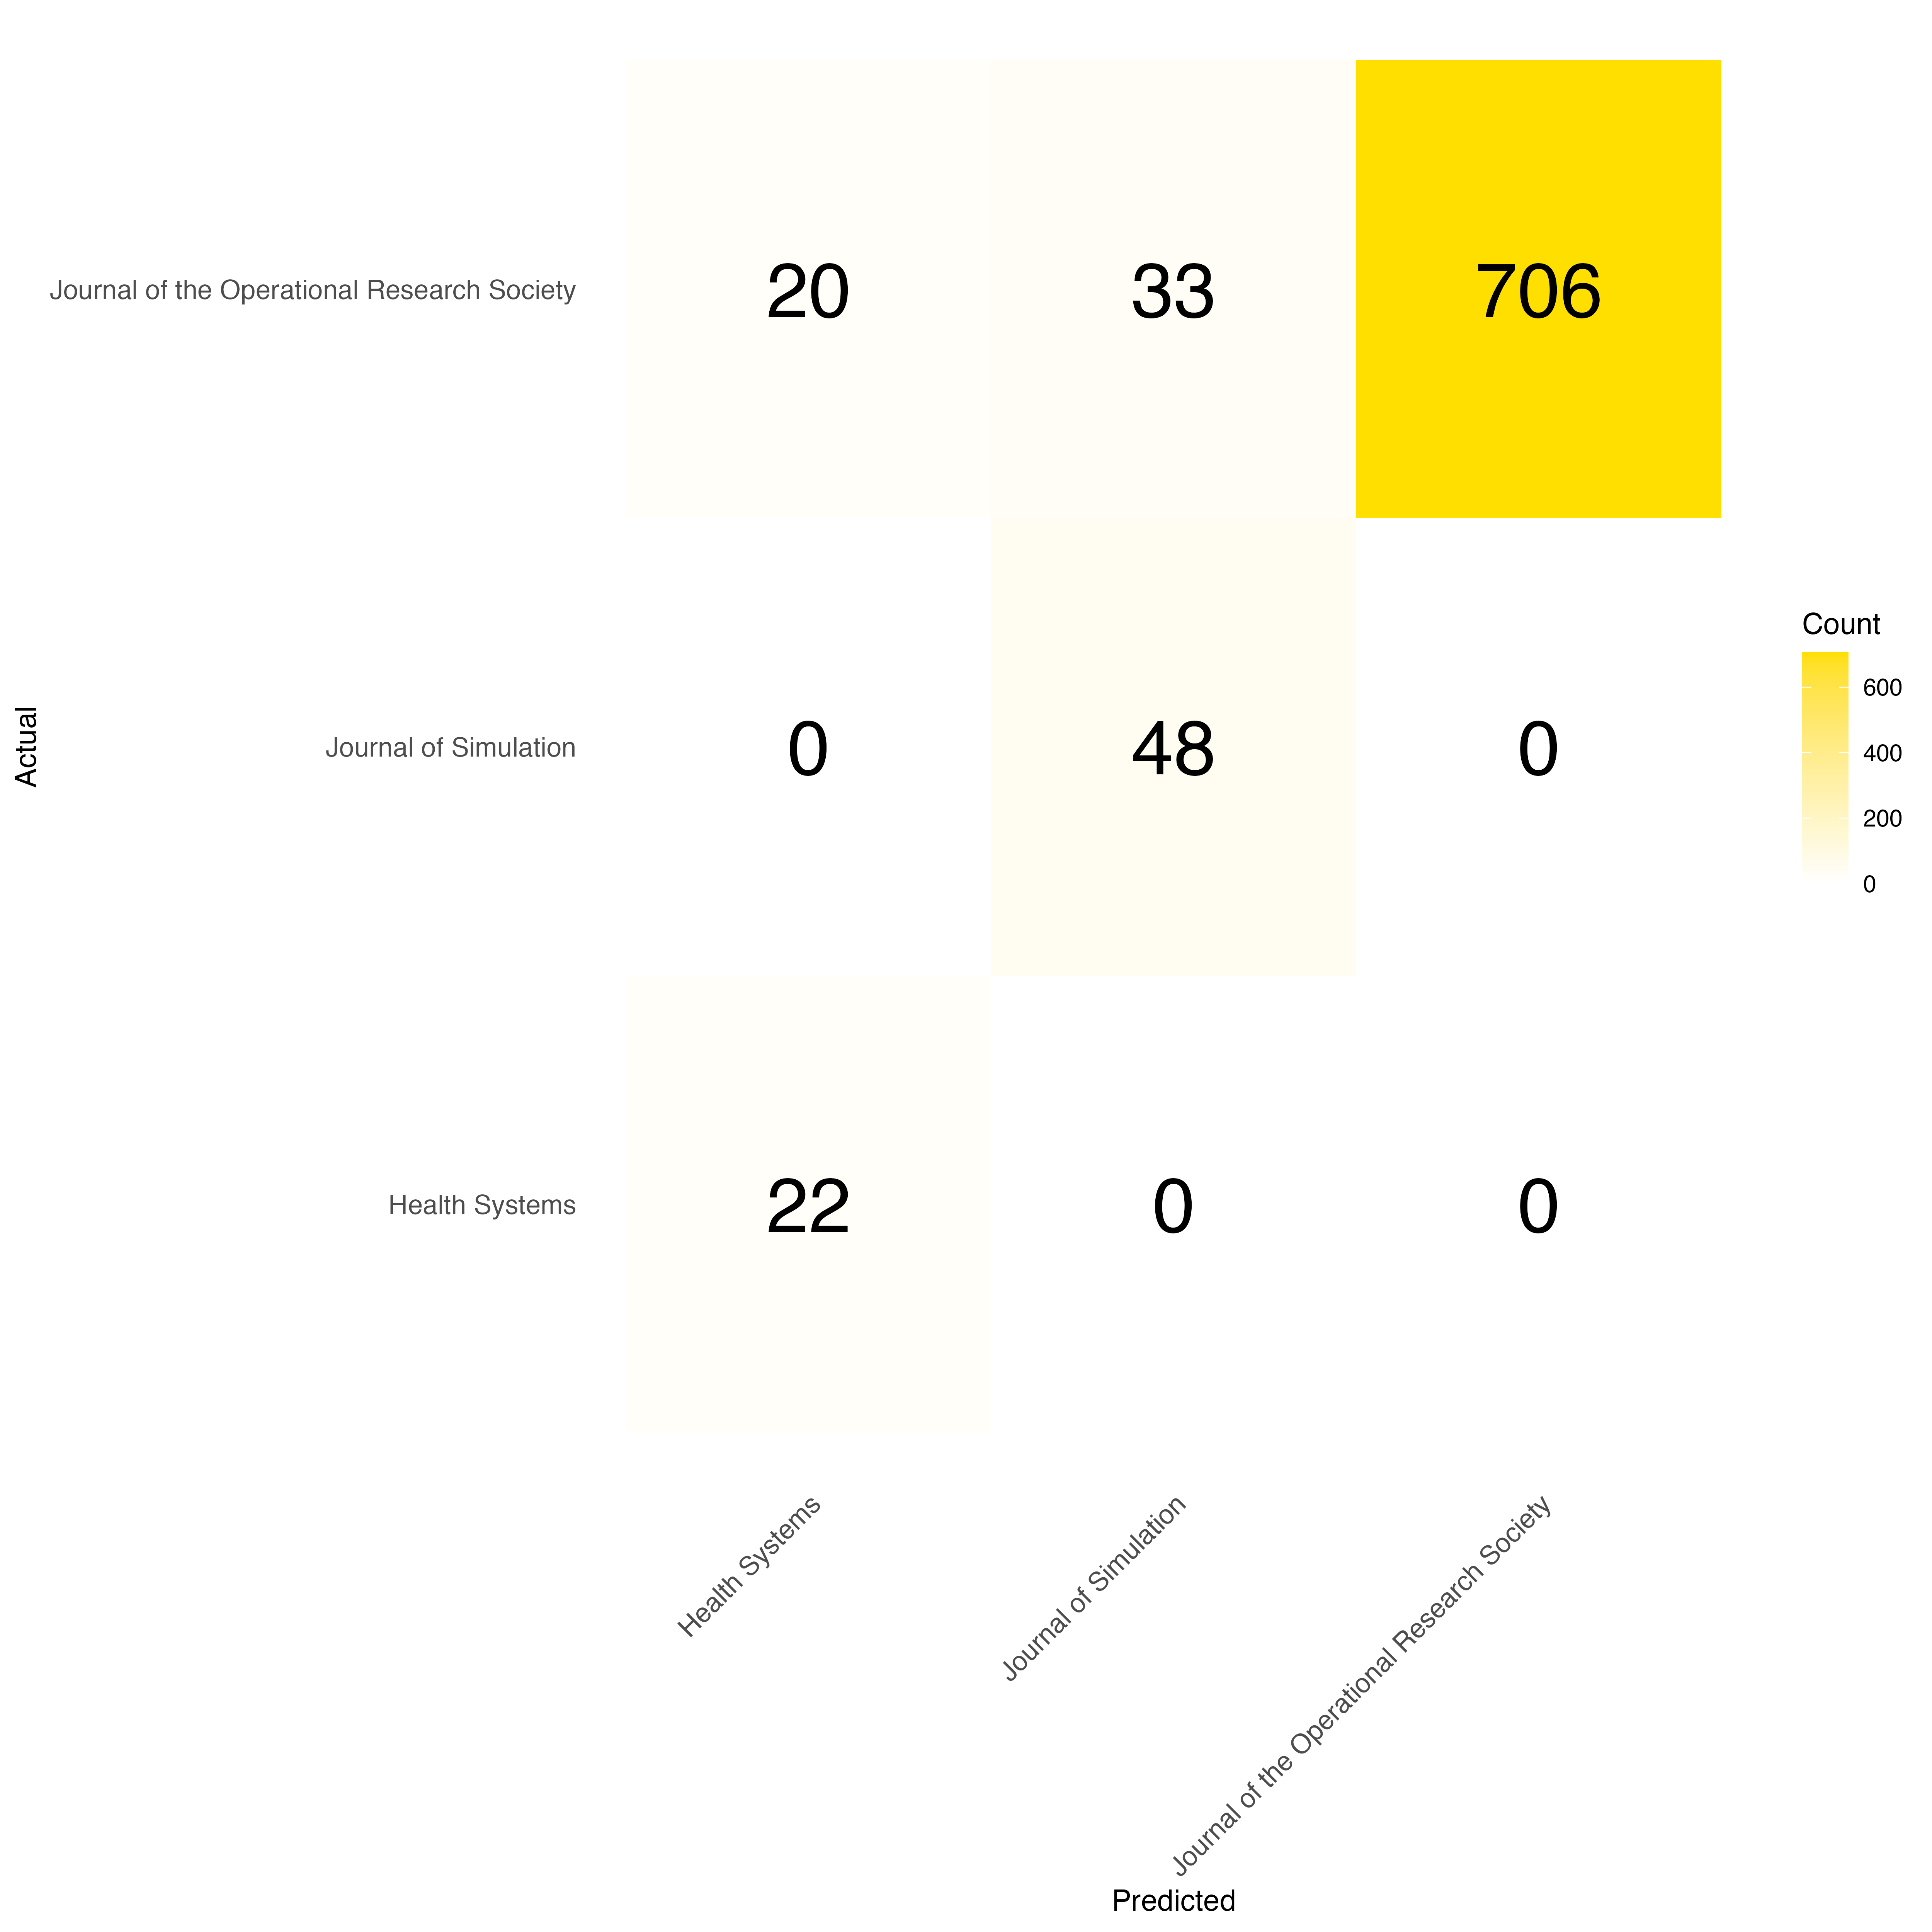
\includegraphics[width=.3\linewidth]{class/conf_SVM.png}
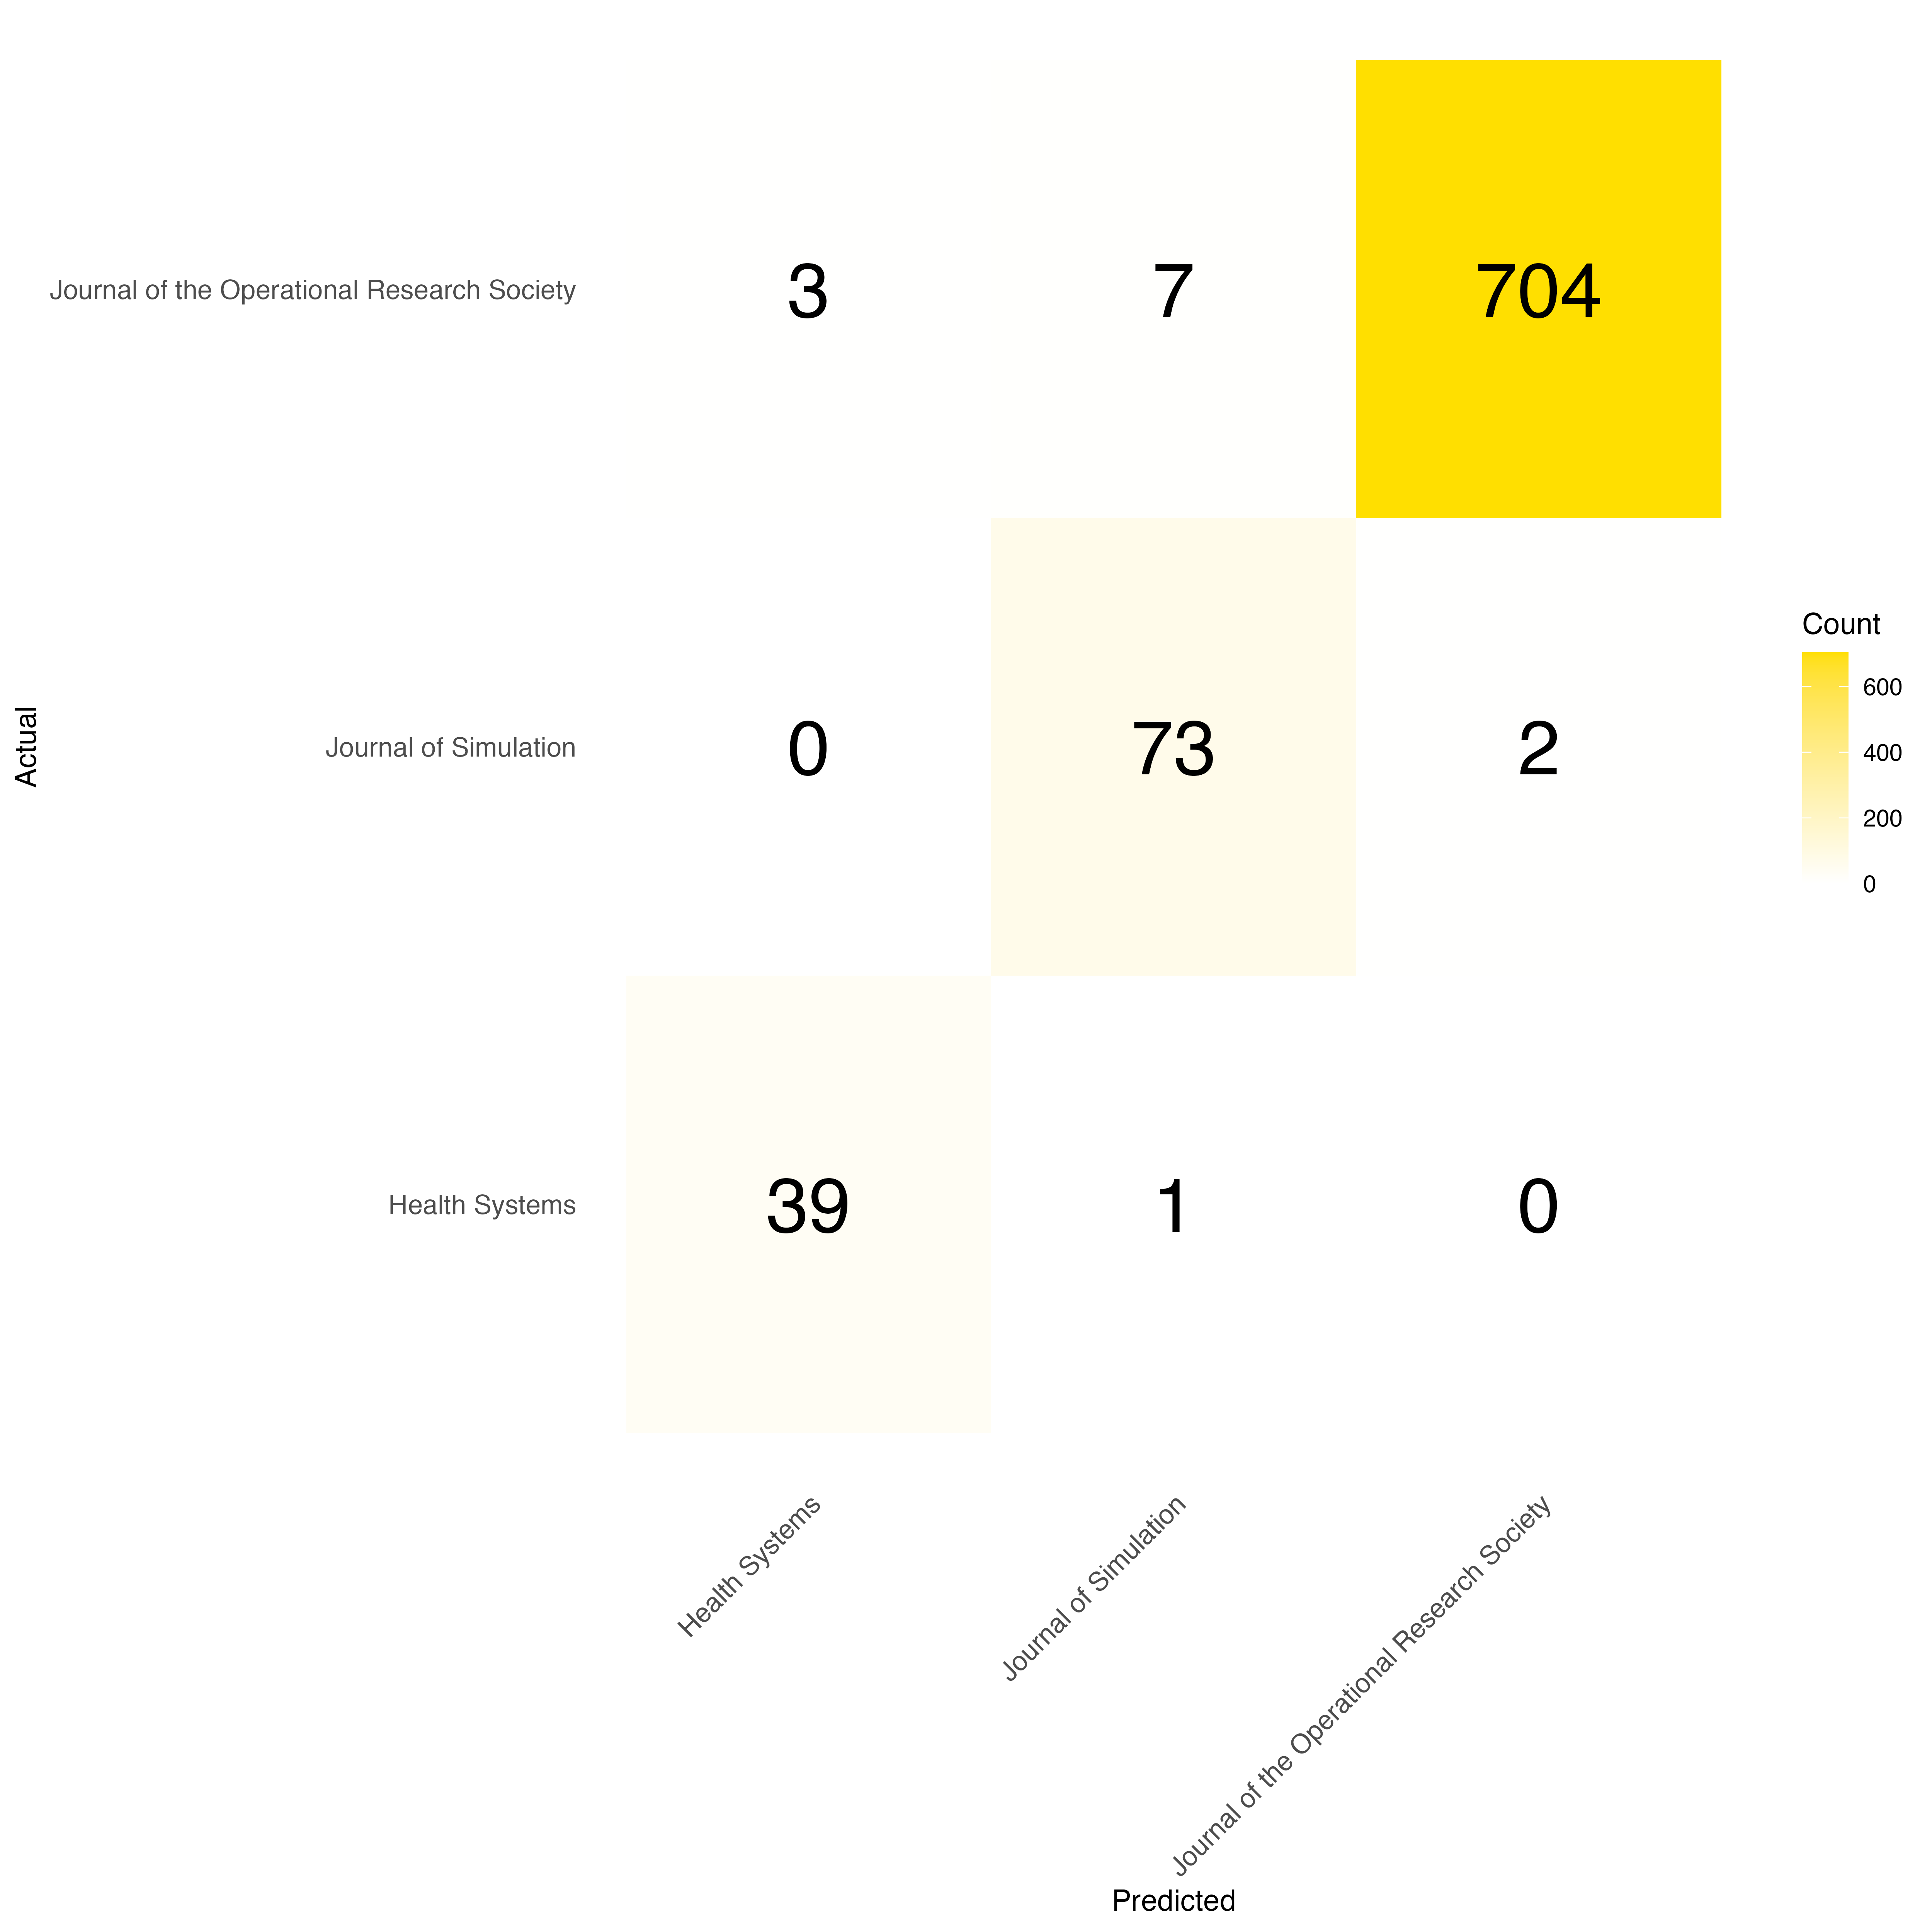
\includegraphics[width=.3\linewidth]{class/conf_XGBoost.png}
\caption{Confusion matrices for RF, SVM, and XGBoost models.}
\label{fig:class_con}
\end{figure}

\subsubsection*{XGBoost}

For the classification task, the XGBoost model was trained with the same parameter settings as in the regression task, including a maximum tree depth of 6, a learning rate ($\eta$) of 0.3, and 100 boosting rounds. The objective function was set to multi-class classification (softmax) to handle the multi-class journal prediction task.

\subsubsection*{SVM}
Support Vector Machine (SVM)~\cite{708428} is a supervised learning algorithm that finds an optimal hyperplane to separate different classes in a high-dimensional feature space. In this study, a radial basis function (RBF) kernel was employed to allow for non-linear decision boundaries, enhancing the model's ability to capture complex relationships in the data. 

\subsubsection*{Neural Network}
A neural network (NN)~\cite{mcculloch1943logical} model is a supervised learning algorithm that models complex relationships between input features and target labels through interconnected layers of neurones. The network architecture in this work consisted of two hidden layers, with 10 neurones in the first layer and 5 neurones in the second layer. The activation function used was sigmoid, ensuring non-linear transformations of the input features. 


\begin{figure}%[tbhp]
\centering
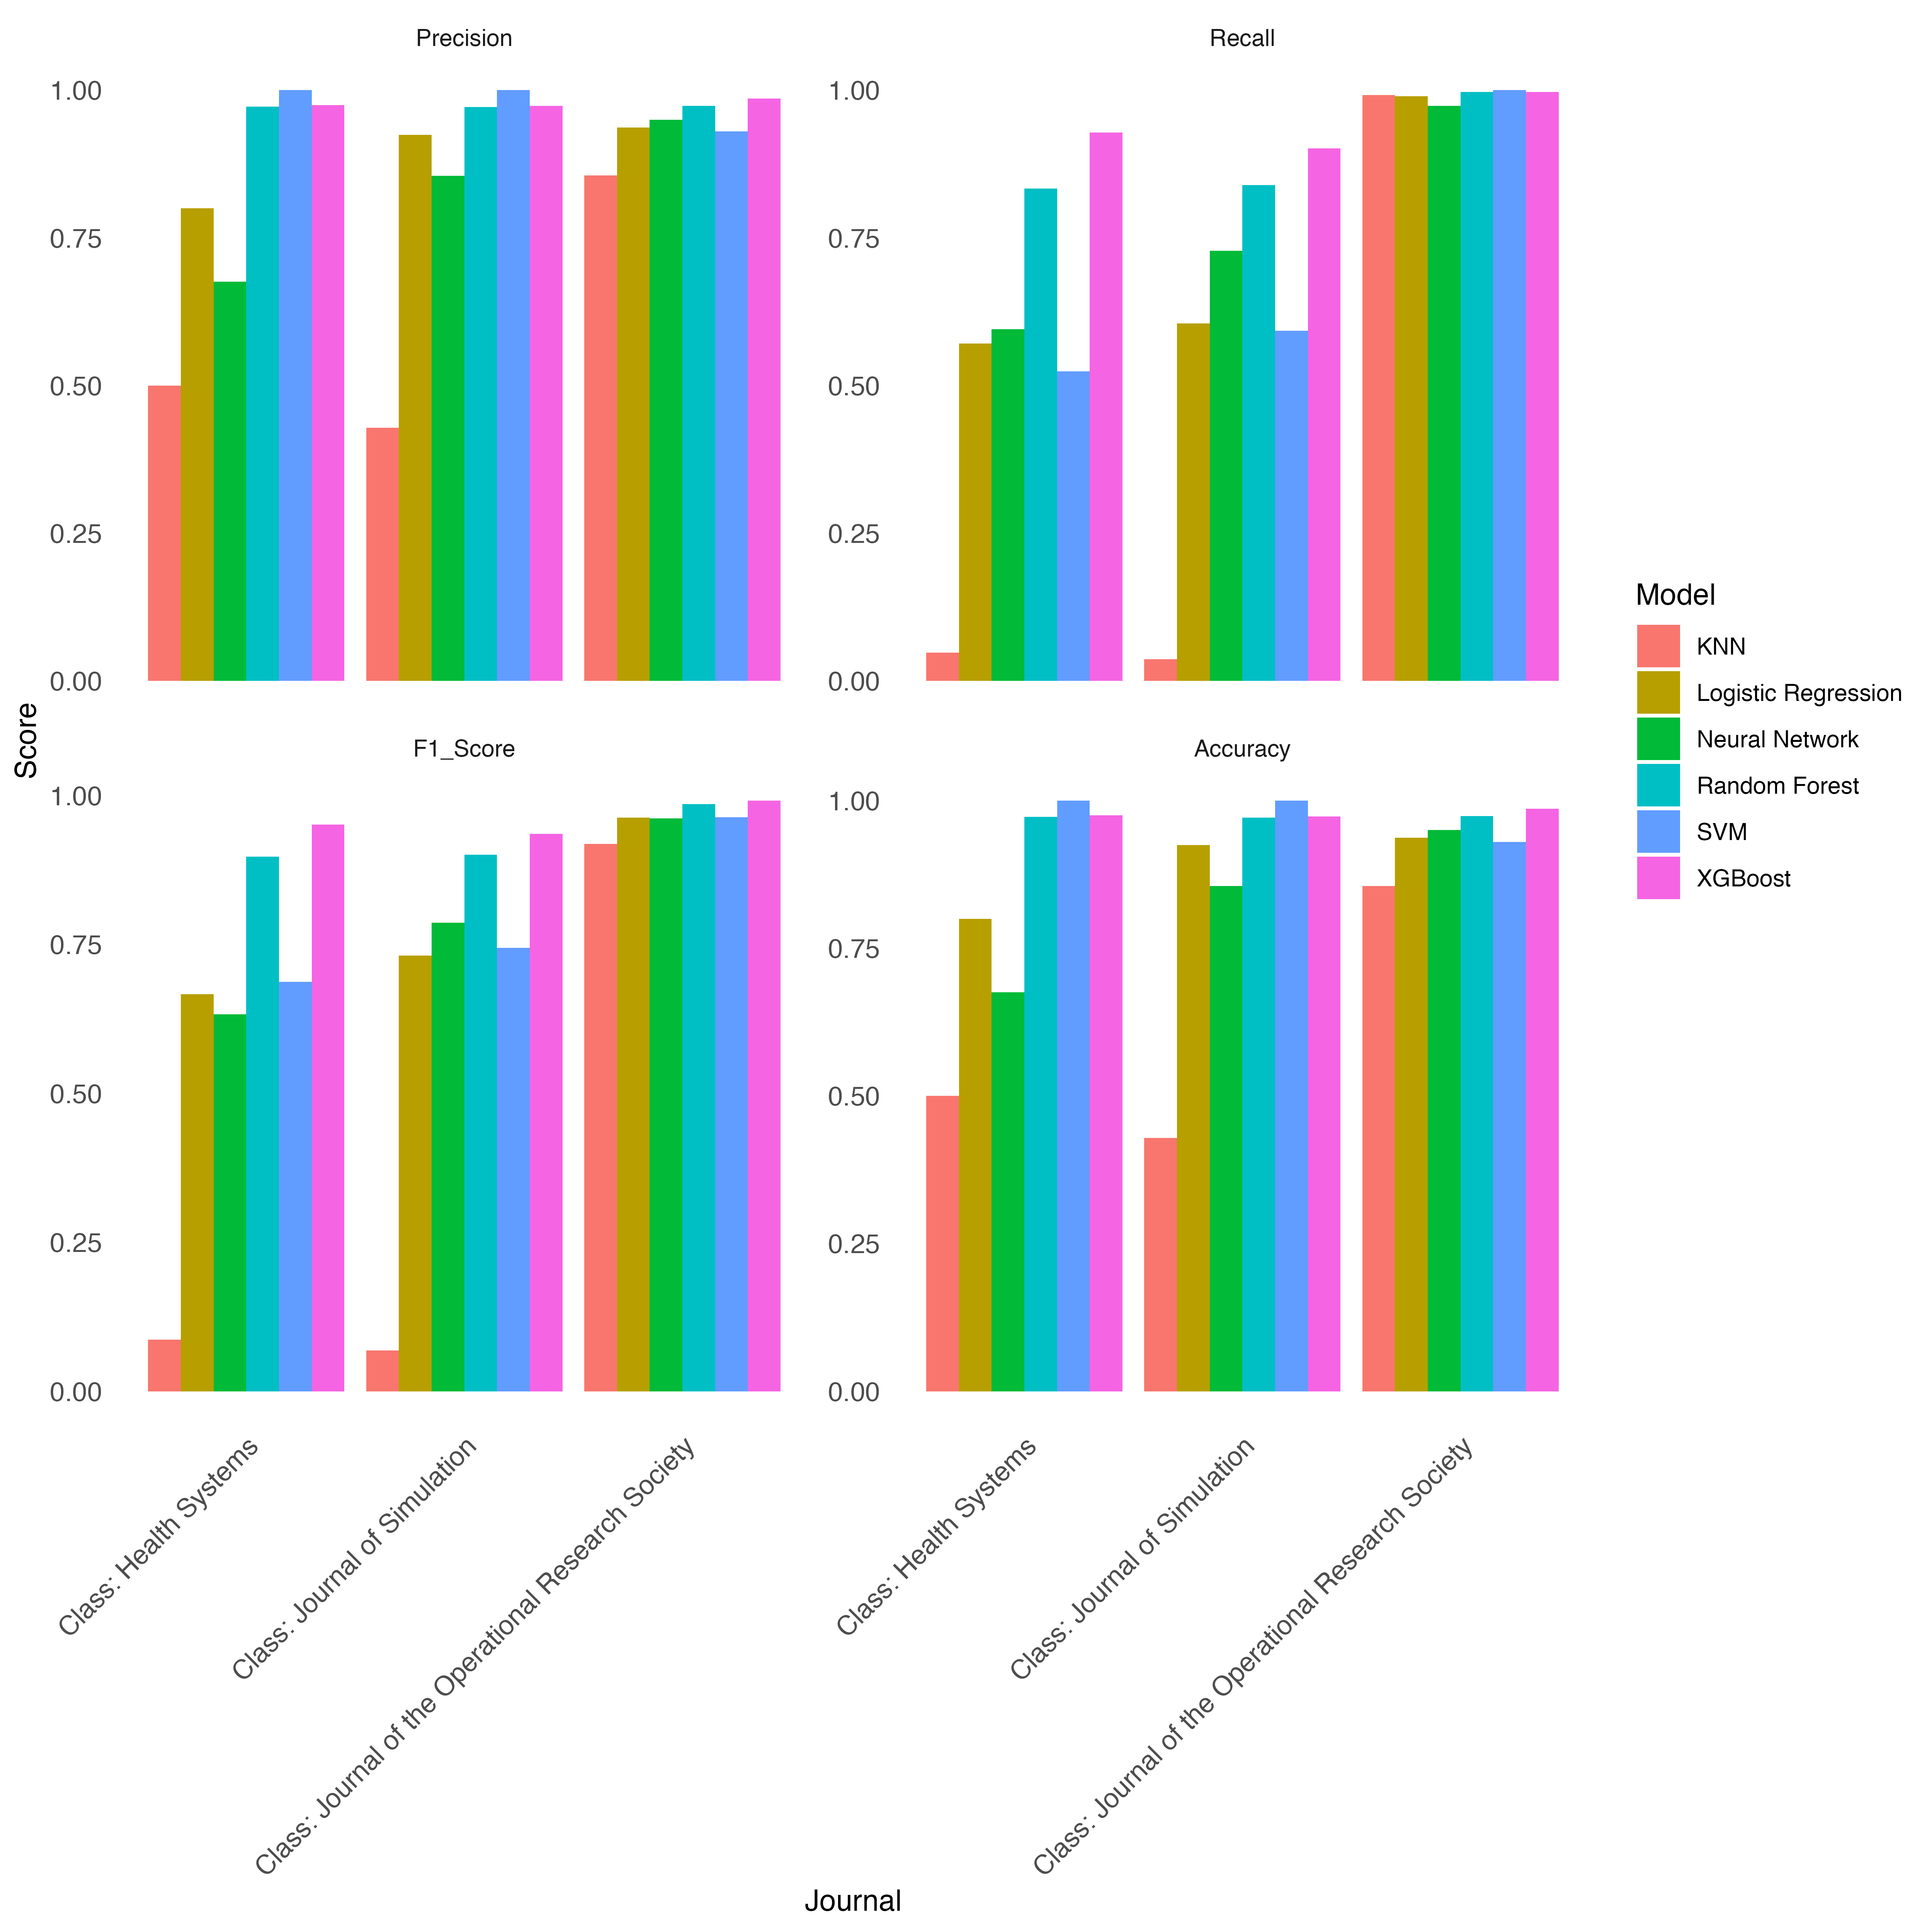
\includegraphics[width=.9\linewidth]{regression/class_metrics_all.png}
\caption{Metrics for classification evaluation.}
\label{fig:class_metrics_all}
\end{figure}


\subsection*{Evaluations}

The RF, SVM, and XGBoost models have the highest accuracy and precision scores, both exceeding 95\%, compared to the other three models as shown in Figure~\ref{fig:class_metrics_all} and Figure~\ref{fig:class_con}. While SVM demonstrated the highest precision across all three models, it showed poorer recall performance for minority samples in the \textit{Health Systems} and \textit{Journal of Simulation categories}.


\section{Prediction Dashboard}

After training, we have one LR model for missing value, two topic models (STM and LDA), 




\acknow{Please include your acknowledgments here, set in a single paragraph. Please do not include any acknowledgments in the Supporting Information, or anywhere else in the manuscript.}

\showacknow % Display the acknowledgements section

% Bibliography
\bibliography{pnas-sample}

\end{document}
